% ********** Rozdział 2 **********
\chapter{Opis struktury projektu}

Niniejszy rozdział przedstawia zaprojektowaną strukturę projektu, 
jego opis techniczny oraz kluczowe informacje dotyczące używanych technologii. 

\section{Język i narzędzia}
Projekt został zrealizowany w języku C\# w platformie .NET 8.0. Wykorzystano również następujące narzędzia:
\begin{itemize}
    \item \textbf{JetBrains Rider} - IDE do programowania w C\#.
    \item \textbf{Newtonsoft.Json} - biblioteka do obsługi JSON.
    \item \textbf{Spectre.Console} - biblioteka do tworzenia interaktywnych konsolowych aplikacji.
    \item \textbf{KanbanFlow} - narzędzie do planowania i zarządzania projektem metodą Kanban.
    \item \textbf{Microsoft Office} - wielozadaniowy pakiet aplikacji biurowych. 
    W projekcie zostały konkretnie wykorzystane programy Word oraz Excel, do projektu gry i 
    przechowywania informacji o mechanikach.
\end{itemize}

\section{Minimalne wymagania sprzętowe}
Aby uruchomić projekt, wymagane są następujące minimalne zasoby sprzętowe:
\begin{itemize}
    \item Procesor: 2.0 GHz lub szybszy.
    \item Pamięć RAM: 4 GB.
    \item Miejsce na dysku: 10 MB wolnego miejsca.
    \item System operacyjny: Windows 10 lub nowszy.
    \item .NET: 8.0 lub nowszy.
\end{itemize}

\section{Zarządzanie danymi}
Zarządzanie danymi w projekcie odbywa się za pomocą plików JSON, które przechowują informacje o postaciach, 
przedmiotach oraz lokacjach. Wykorzystano klasę \texttt{DataPersistanceManager} do odczytu i zapisu stanu gry, 
co umożliwia łatwe zarządzanie stanem gry. Ponadto, dane o obiektach stałych, takich jak przeciwnicy, przedmioty, 
czy tablice dropów przechowywane są w formacie JSON do deserializacji poprzez użycie metod zarządzających w klasach, 
takich jak \texttt{PlantDropManager} czy \texttt{ItemManager}. W celu deserializacji list obiektów używających interfejsów, stworzono
specjalne konwertery przy użyciu Biblioteki Newtonsoft.Json.


\section{Diagram klas}
W tej sekcji przedstawiono diagram klas projektu, w celu wizualizacji struktury klas i ich pola, własciwości oraz metody.
Ze względu na duży rozmiar projektu i powstałego diagramu klas, podzielono diagram na sekcje, każda odpowiadająca za osobny podfolder struktury.
\begin{itemize}
    \item Na rysunku 2.1, przedstawiono sekcję Characters (Postacie), odpowiedzialną za klasy postaci gracza i przeciwników.
        \begin{figure}[H]
        \centering
        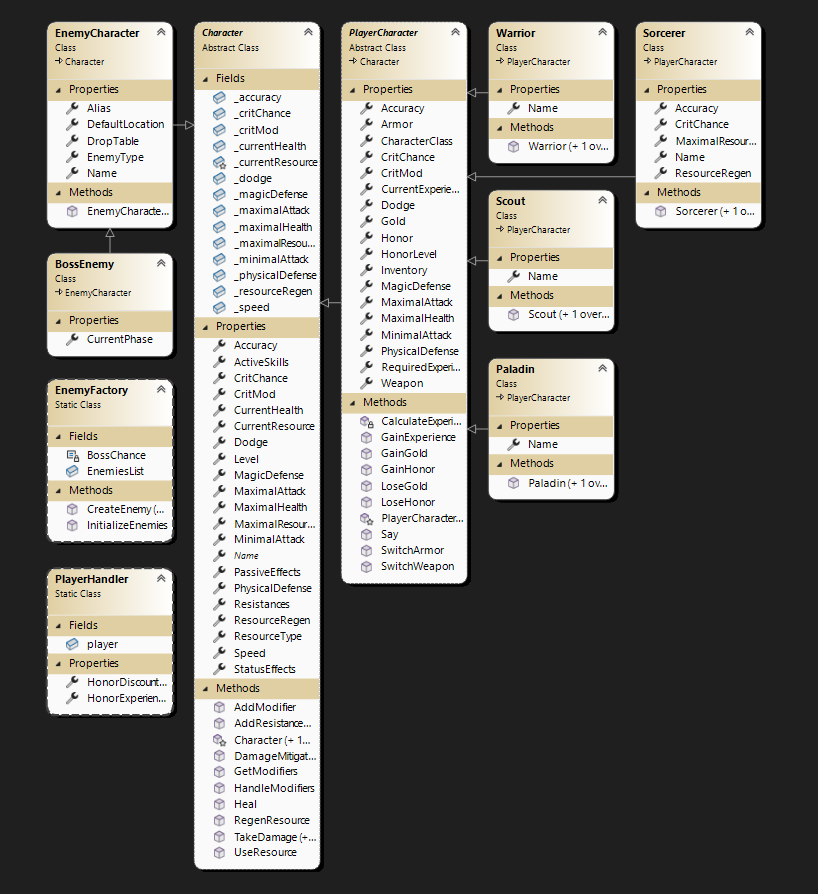
\includegraphics[width=0.8\textwidth]{figures/class_diagram_characters.png}
        \caption{Diagram klas przedstawiający strukturę części `Characters' projektu.}
        \label{fig:class_diagram_characters}
        \end{figure}

    \begin{minipage}{\linewidth}%
    \item Na rysunku 2.2, przedstawiono sekcję Combat (Walka), odpowiedzialną za klasy używane przez mechaniki systemu walki: umiejętności, statystyki, bitwy oraz efekty pasywne.
        \begin{figure}[H]
        \centering
        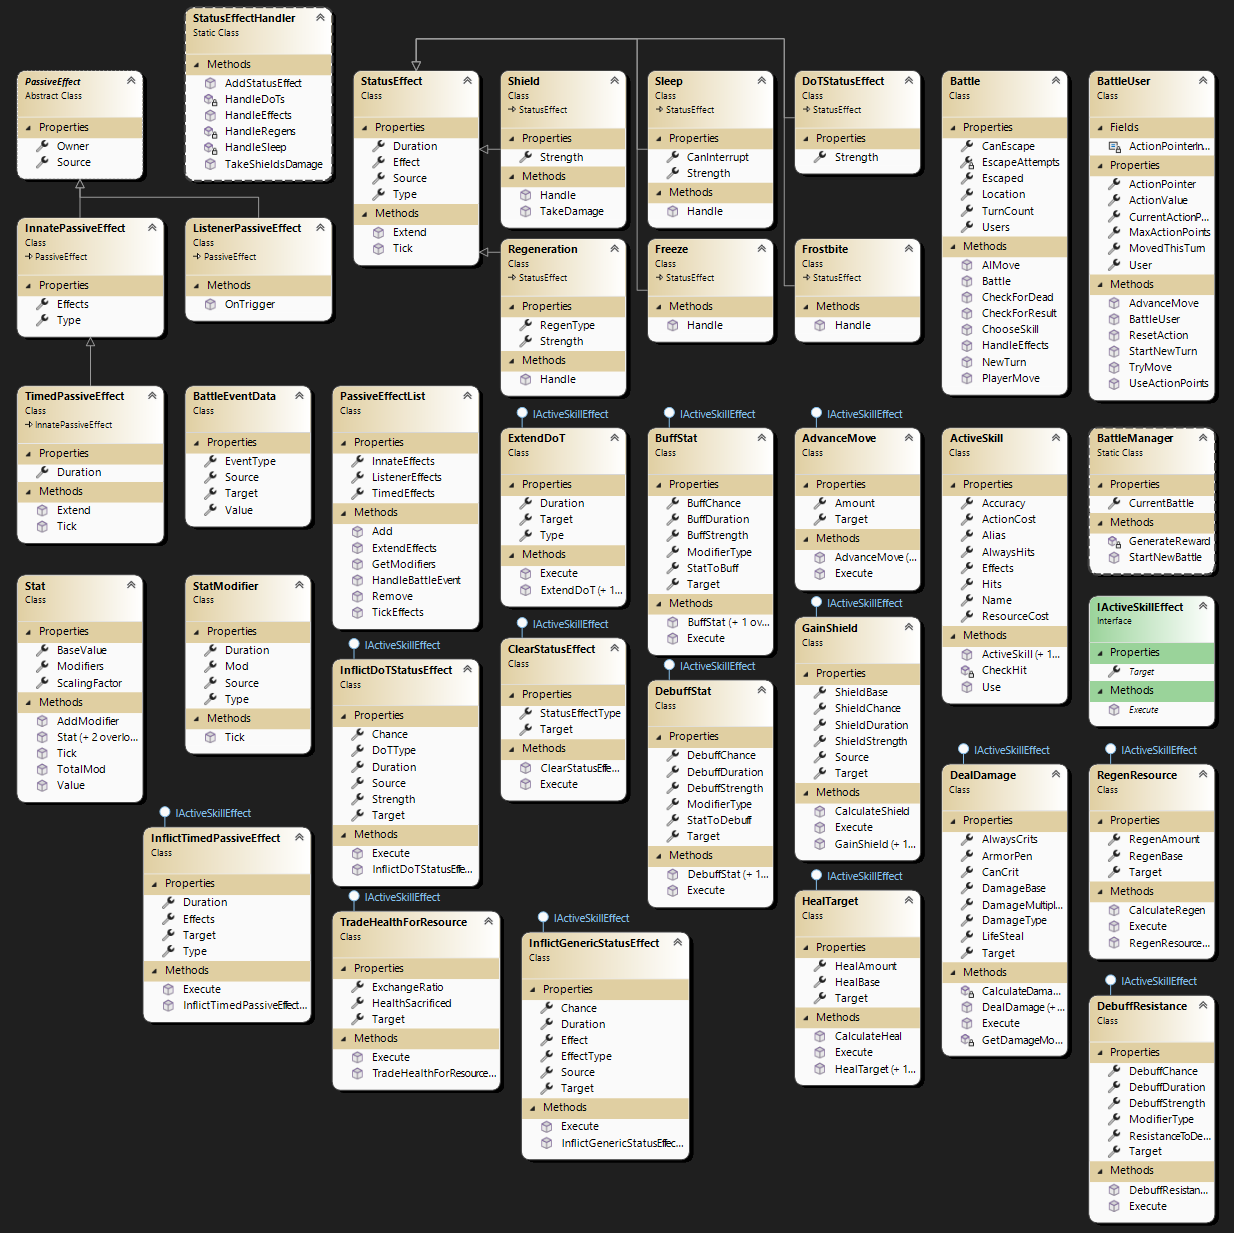
\includegraphics[width=0.8\textwidth]{figures/class_diagram_combat.png}
        \caption{Diagram klas przedstawiający strukturę części `Combat' projektu.}
        \label{fig:class_diagram_combat}
        \end{figure}
    \end{minipage}

    \begin{minipage}{\linewidth}%
    \item Na rysunku 2.3, przedstawiono sekcję Dungeons (Lochy), odpowiedzialną za klasy umożliwiające eksplorację i generowanie lochów.
        \begin{figure}[H]
        \centering
        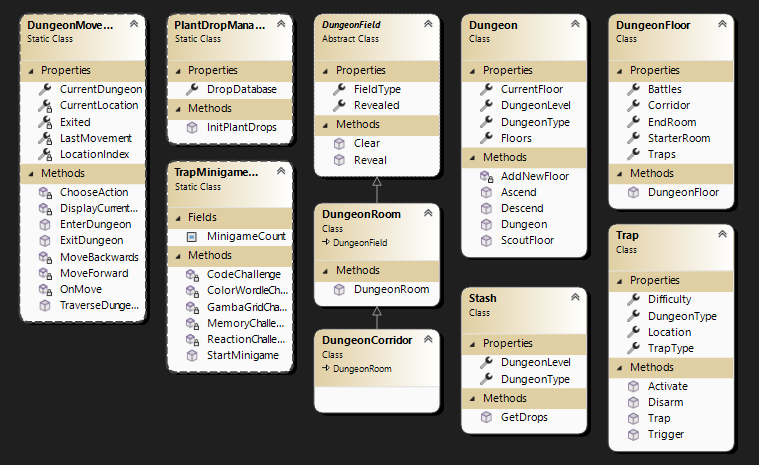
\includegraphics[width=0.8\textwidth]{figures/class_diagram_dungeons.png}
        \caption{Diagram klas przedstawiający strukturę części `Dungeons' projektu.}
        \label{fig:class_diagram_dungeons}
        \end{figure}
    \end{minipage}
    
    \begin{minipage}{\linewidth}%
    \item Na rysunku 2.4, przedstawiono sekcję Enums (Enumy), odpowiedzialną za przechowywanie typów wyliczeniowych projektu.
        \begin{figure}[H]
        \centering
        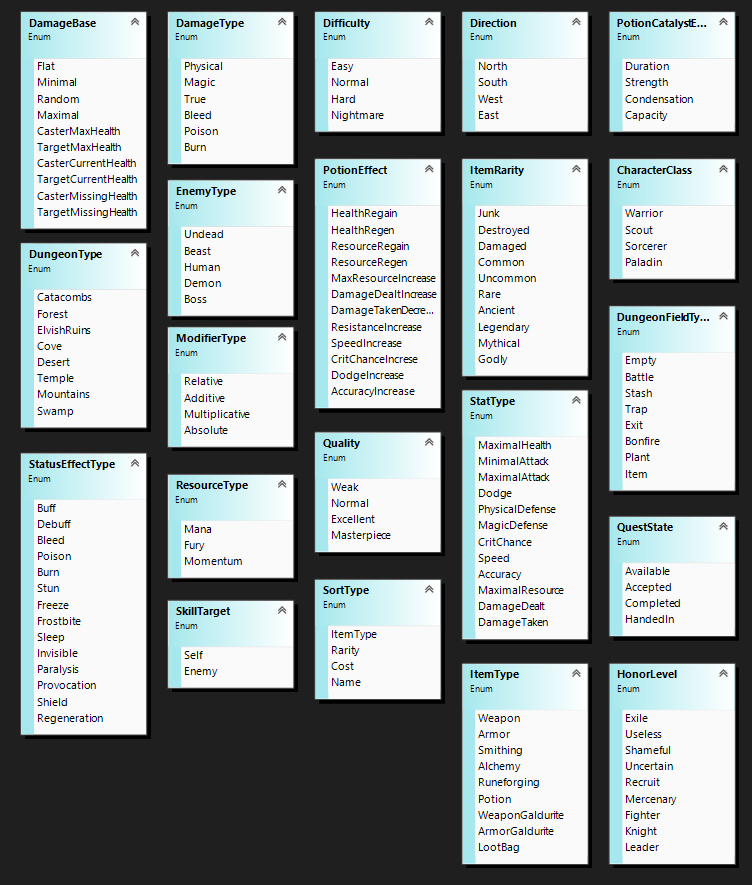
\includegraphics[width=0.8\textwidth]{figures/class_diagram_enums.png}
        \caption{Diagram klas przedstawiający strukturę części `Enums' projektu.}
        \label{fig:class_diagram_enums}
        \end{figure}
    \end{minipage}

    \begin{minipage}{\linewidth}%
    \item Na rysunku 2.5, przedstawiono sekcję Items (Przedmioty), odpowiedzialną za klasy implementujące typy przedmiotów i zarządzające nimi.
        \begin{figure}[H]
        \centering
        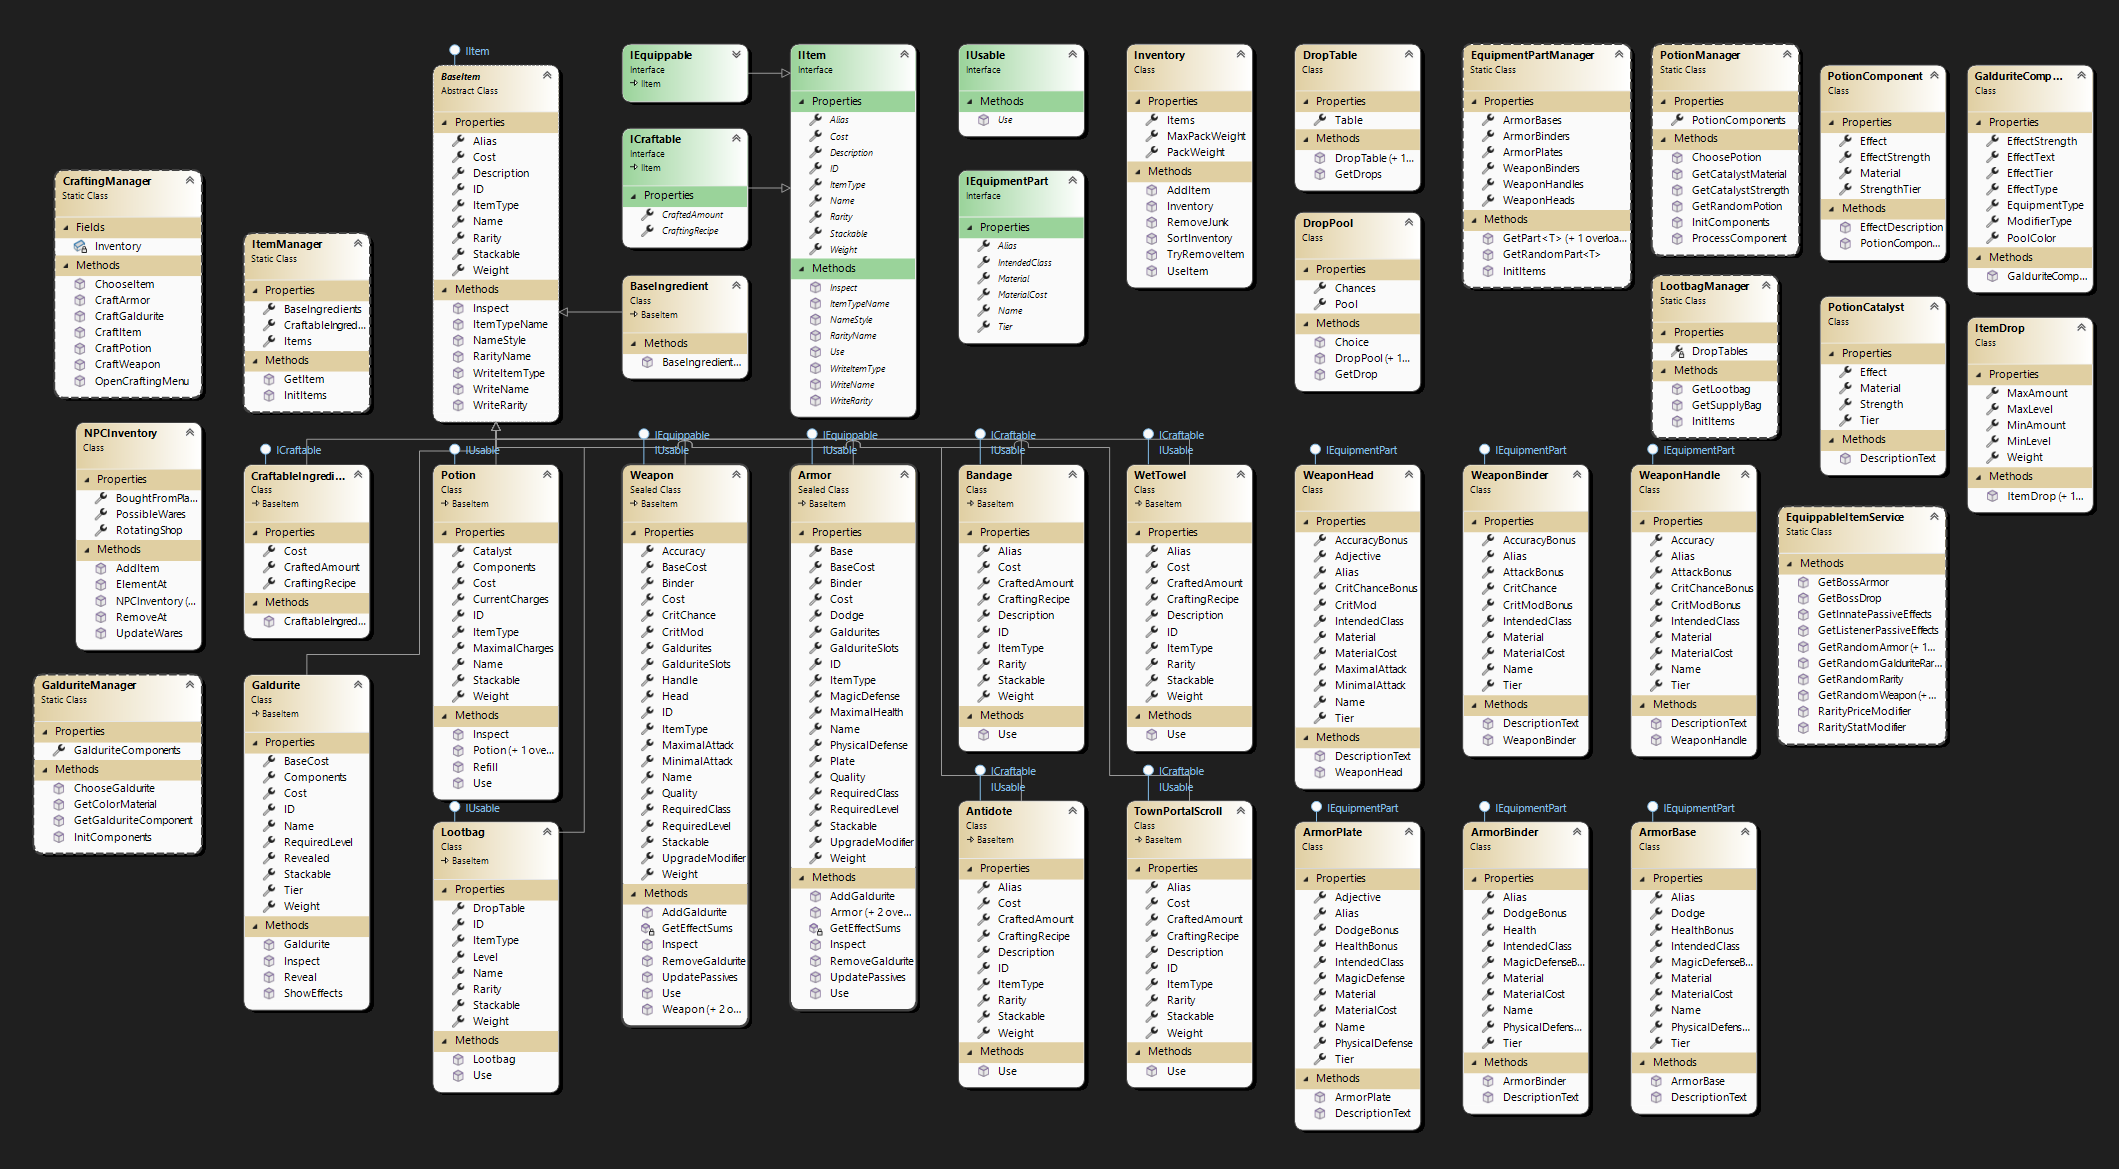
\includegraphics[width=0.8\textwidth]{figures/class_diagram_items.png}
        \caption{Diagram klas przedstawiający strukturę części `Items' projektu.}
        \label{fig:class_diagram_items}
        \end{figure}
    \end{minipage}

    \begin{minipage}{\linewidth}%
    \item Na rysunku 2.6, przedstawiono sekcję Quests (Zadania), odpowiedzialną za klasy implementujące strukturę zadań i zarządzające nimi.
        \begin{figure}[H]
        \centering
        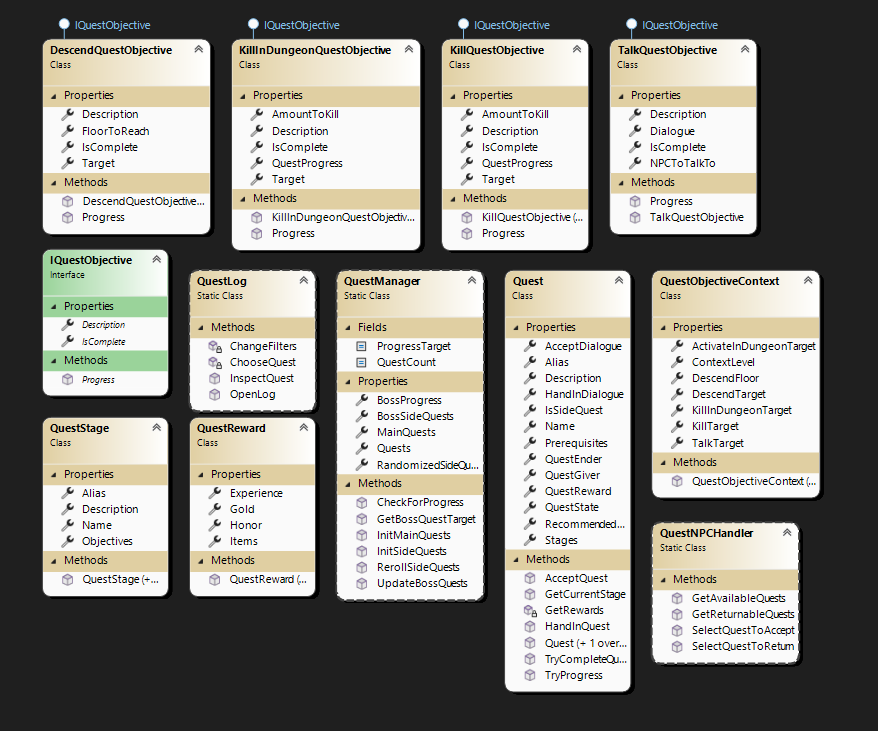
\includegraphics[width=0.8\textwidth]{figures/class_diagram_quests.png}
        \caption{Diagram klas przedstawiający strukturę części `Quests' projektu.}
        \label{fig:class_diagram_quests}
        \end{figure}
    \end{minipage}

    \begin{minipage}{\linewidth}%
    \item Na rysunku 2.7, przedstawiono sekcję Text (Tekst), odpowiedzialną za klasy zarządzające tekstem, wyświetlaniem go na ekranie, oraz nawigacją po menu.
        \begin{figure}[H]
        \centering
        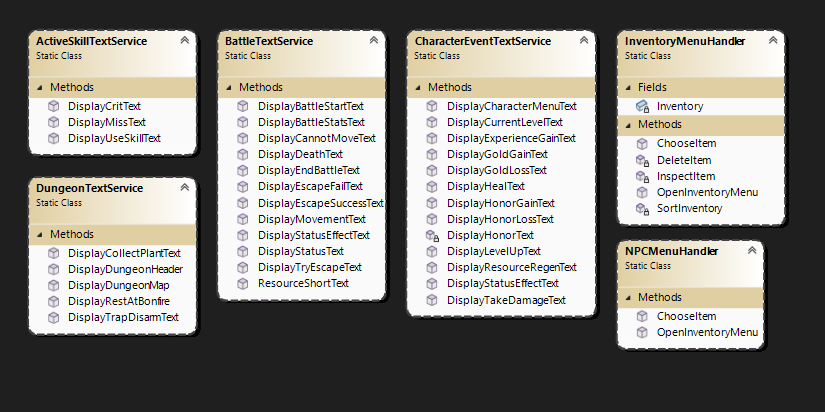
\includegraphics[width=0.8\textwidth]{figures/class_diagram_text.png}
        \caption{Diagram klas przedstawiający strukturę części `Text' projektu.}
        \label{fig:class_diagram_text}
        \end{figure}
    \end{minipage}

    \begin{minipage}{\linewidth}%
    \item Na rysunku 2.8, przedstawiono sekcję Towns (Miasta), odpowiedzialną za klasy postaci niezależnych oraz miast.
        \begin{figure}[H]
        \centering
        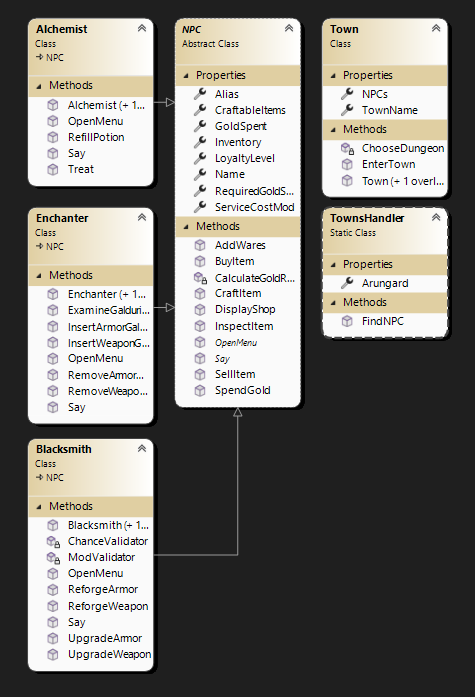
\includegraphics[width=0.8\textwidth]{figures/class_diagram_towns.png}
        \caption{Diagram klas przedstawiający strukturę części `Towns' projektu.}
        \label{fig:class_diagram_towns}
        \end{figure}
    \end{minipage}

    \begin{minipage}{\linewidth}%
    \item Na rysunku 2.9, przedstawiono sekcję Utilities (Narzędzia), odpowiedzialną za inne narzędzia pomocnicze i systemy, takie jak konwertery JSON, czy przydatne metody rozszerzające.
        \begin{figure}[H]
        \centering
        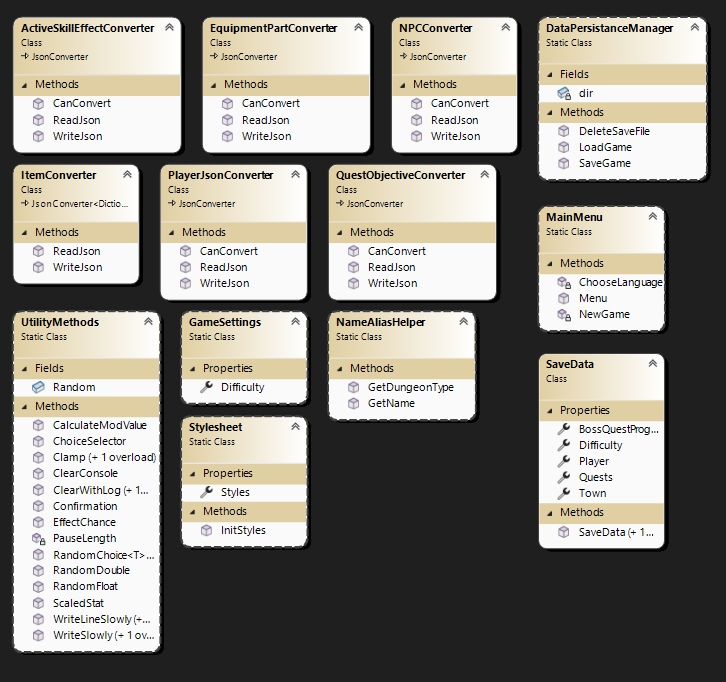
\includegraphics[width=0.8\textwidth]{figures/class_diagram_utilities.png}
        \caption{Diagram klas przedstawiający strukturę części `Utilities' projektu.}
        \label{fig:class_diagram_utilities}
        \end{figure}
    \end{minipage}
\end{itemize}


\section{Hierarchia i opisy klas}
Projekt zawiera złożoną hierarchię klas, która umożliwia efektywne zarządzanie postaciami, 
przedmiotami oraz interakcjami w grze. Poniżej przedstawiono klasy oraz ich najważniejsze metody:

\begin{itemize}
    \item \textbf{Character} - abstrakcyjna klasa bazowa dla wszystkich postaci w grze. 
    Odpowiada za zarządzanie podstawowymi właściwościami postaci, takich jak zdrowie, 
    atak czy obrona oraz na interakcje z otoczeniem. Najwazniejsze metody:
        \begin{itemize}
            \item \texttt{TakeDamage(double damage, dynamic source)} - metoda do obliczania przyjętych obrażeń 
            i odejmowaniu ich od zdrowia.
            \item \texttt{Heal(double heal)} - metoda do leczenia postaci.
            \item \texttt{UseResource(int amount)}: Używa określoną ilość zasobu (many, pędu lub wściekłości).
            \item \texttt{RegenResource(int amount)}: Regeneruje określoną ilość zasobu.
            \item \texttt{AddModifier(StatType stat, StatModifier modifier)}: Dodaje modyfikator do określonej statystyki postaci.
            \item \texttt{HandleModifiers()} : Obsługuje modyfikatory postaci, aktualizując ich czas trwania.
        \end{itemize}
        \item \textbf{PlayerCharacter} - klasa dziedzicząca po \texttt{Character}, reprezentująca postać gracza. 
        Odpowiada za zarządzanie unikalnymi właściwościami i umiejętnościami gracza. Najważniejsze metody:
            \begin{itemize}
                \item \texttt{SwitchWeapon(Weapon weapon)} - zmienia aktualnie używaną broń postaci na podaną. 
                Jeśli postać ma już broń, dodaje ją do ekwipunku.
                \item \texttt{SwitchArmor(Armor armor)} - zmienia aktualnie używaną zbroję postaci na podaną. 
                Jeśli postać ma już zbroję, dodaje ją do ekwipunku i aktualizuje zdrowie postaci.
                \item \texttt{GainGold(int gold)} - przyznaje postaci określoną ilość złota, uwzględniając modyfikatory 
                pasywne dotyczące zdobywania złota.
                \item \texttt{LoseGold(int gold)} - odejmuje określoną ilość złota od postaci.
                \item \texttt{GainExperience(int experience)} - przyznaje postaci doświadczenie, co może prowadzić do 
                awansu na wyższy poziom. Aktualizuje zdrowie postaci po awansie.
                \item \texttt{GainHonor(int honor)} - przyznaje postaci honor, nie przekraczając maksymalnego limitu.
                \item \texttt{LoseHonor(int honor)} - odejmuje honor od postaci, nie przekraczając minimalnego limitu.
                \item \texttt{Say(string message)} - wyświetla wiadomość postaci w formacie dialogowym.
            \end{itemize}
        \item \textbf{PlayerHandler} - statyczna klasa odpowiedzialna za zarządzanie stanem i interakcjami postaci gracza w grze. 
        Przechowuje aktualny obiekt gracza w statycznym polu publicznym. Nie posiada żadnych metod.
        \item \textbf{Warrior, Rogue, Mage i Paladin} - klasy dziedziczące po \texttt{PlayerCharacter} służące do tworzenia obiektów konkretnej klasy postaci gracza. 
        Posiadają konstruktor wypełniony wartościami bazowymi. Nie posiadają żadnych metod.
        \item \textbf{EnemyCharacter} - klasa dziedzicząca po \texttt{Character}, reprezentująca przeciwnika w grze. 
        Odpowiada za zarządzanie unikalnymi właściwościami i zachowaniami przeciwników. Nie posiada żadnych metod.
        \item \textbf{EnemyFactory} - statyczna klasa odpowiedzialna za tworzenie instancji przeciwników w grze. 
        Zarządza listą dostępnych przeciwników oraz logiką ich generowania. Najważniejsze metody:
            \begin{itemize}
                \item \texttt{CreateEnemy(string alias, int level)} - metoda, która tworzy konkretnego przeciwnika na podstawie podanego aliasu 
                oraz poziomu. Wyszukuje przeciwnika w liście i zwraca nową instancję z odpowiednim poziomem.
                \item \texttt{CreateEnemy(DungeonType dungeonType, int level)} - metoda, która generuje losowego przeciwnika na podstawie typu lochu 
                oraz poziomu. Sprawdza, czy można wygenerować bossa, a jeśli nie, wybiera losowego przeciwnika z dostępnych w danym lochu.
                \item \texttt{InitializeEnemies()} - metoda inicjalizująca listę przeciwników poprzez wczytanie danych z pliku JSON. 
                Sprawdza, czy plik istnieje, a następnie deserializuje dane do listy przeciwników.
            \end{itemize}
        \item \textbf{BossEnemy} - klasa dziedzicząca po \texttt{EnemyCharacter}, reprezentująca bossa w grze. 
        Odpowiada za zarządzanie unikalnymi właściwościami i zachowaniami bossów. Nie posiada żadnych metod.
        \item \textbf{Battle} - klasa odpowiedzialna za zarządzanie przebiegiem walki w grze. 
        Odpowiada za interakcje między postaciami gracza a przeciwnikami, zarządzanie turami oraz wynikami walki. Najważniejsze metody:
            \begin{itemize}
                \item \texttt{NewTurn()} - metoda, która rozpoczyna nową turę walki, resetując stany użytkowników i umożliwiając im wykonanie akcji.
                \item \texttt{HandleEffects(BattleUser user)} - obsługuje efekty statusowe oraz regenerację zasobu dla podanego użytkownika.
                \item \texttt{ChooseSkill(BattleUser player, BattleUser target)}- daje graczowi wybór umiejętności do użycia na wybranym celu.
                \item \texttt{PlayerMove(BattleUser player, BattleUser target)} - obsługuje ruch gracza, pozwalając na wykonanie akcji, takich jak użycie 
                umiejętności lub przedmiotu czy ucieczkę z walki.
                \item \texttt{AIMove(BattleUser enemy, BattleUser target)} - obsługuje ruch przeciwnika, wybierając odpowiednie umiejętności do użycia.
                \item \texttt{CheckForResult()} - sprawdza wynik walki, określając, czy gracz, czy przeciwnik wygrał, czy też może gracz uciekł.
                \item \texttt{CheckForDead()} - sprawdza, które postacie są martwe, aktualizując stan walki i usuwając martwych użytkowników z walki.
            \end{itemize}
        \item \textbf{BattleManager} - statyczna klasa odpowiedzialna za zarządzanie stanem aktualnie przebiegającej walki w grze. 
        Zarządza aktualną walką, jej rozpoczęciem, zakońceniem oraz generowaniem nagród po zakończeniu. Najważniejsze metody:
            \begin{itemize}
                \item \texttt{StartNewBattle(Battle battle)} - rozpoczyna nową walkę, resetując stan walki oraz regenerując zasoby użytkowników.
                \item \texttt{GenerateReward(Dictionary<BattleUser, int> usersTeams)} - generuje nagrody dla gracza po zakończeniu walki, przyznając złoto, 
                honor i doświadczenie i przedmiotów podstawie pokonanych przeciwników.
            \end{itemize}
        \item \textbf{BattleUser} - klasa odpowiedzialna za reprezentowanie uczestnika walki walce. 
        Zarządza stanem postaci, punktami akcji oraz interakcjami w trakcie tury. Najważniejsze metody:
            \begin{itemize}
                \item \texttt{ResetAction()} - resetuje punkty akcji oraz wskaźnik akcji uczestnika, przygotowując go do nowej tury.
                \item \texttt{TryMove()} - próbuje wykonać ruch, zmniejszając wartość akcji i sprawdzając, czy użytkownik może się poruszyć.
                \item \texttt{AdvanceMove(int amount)} - zmniejsza wartość akcji o podaną ilość, co pozwala na wcześniejszy ruch w turze.
                \item \texttt{UseActionPoints(double amount)} - zużywa określoną ilość punktów akcji, aktualizując ich bieżącą wartość.
                \item \texttt{StartNewTurn()} - resetuje stan uczestnika na początku nowej tury, przygotowując go do działania.
            \end{itemize}
        \item \textbf{Stat} - klasa odpowiedzialna za zarządzanie statystykami postaci w grze. 
        Zarządza wartościami bazowymi, współczynnikami skalowania oraz modyfikatorami. Najważniejsze metody:
            \begin{itemize}
                \item \texttt{Value(Character owner, string statName)} - metoda, która oblicza i zwraca wartość statystyki, 
                uwzględniając modyfikatory oraz poziom postaci.
                \item \texttt{Tick()} - metoda, która aktualizuje modyfikatory, usuwając te, które wygasły.
                \item \texttt{AddModifier(StatModifier modifier)} - metoda, która dodaje nowy modyfikator do listy modyfikatorów statystyki.
            \end{itemize}
        \item \textbf{StatModifier} - klasa reprezentująca modyfikator statystyk w grze. Odpowiada za przechowywanie informacji o typie modyfikatora,
         jego wartości, źródle oraz czasie trwania. Najważniejsze metody:
            \begin{itemize}
                \item \texttt{Tick()} - metoda, która zmniejsza czas trwania modyfikatora o jeden i usuwa go, jeśli czas trwania osiągnie zero.
            \end{itemize}
        \item \textbf{PassiveEffect} - klasa abstrakcyjna, która reprezentuje pasywne efekty przypisane do postaci w grze. 
        Odpowiada za zarządzanie efektami, które wpływają na statystyki i zachowanie postaci. Nie posiada żadnych metod.
        \item \textbf{BattleEventData} - klasa reprezentująca dane zdarzenia w trakcie walki. 
        Zawiera informacje o typie zdarzenia, źródle oraz celu zdarzenia. Nie posiada żadnych metod.
        \item \textbf{InnatePassiveEffect} - klasa dziedzicząca po \texttt{PassiveEffect}, reprezentująca pasywne efekty, które są przypisane do postaci.
        Efekty te są przypisane oraz działają cały czas, dopóki ich źródło nie zostanie usunięte (broń, umiejętność pasywna). Nie posiada żadnych metod.
        \item \textbf{ListenerPassiveEffect} - klasa reprezentująca pasywny efekt, który reaguje na zdarzenia w grze. Efekty te są przypisane cały czas,
        dopóki ich źródło nie zostanie usunięte, ale efekt aktywuje się dopiero po spełnieniu warunku przez zdarzenie w walce. Najważniejsze metody:
            \begin{itemize}
                \item \texttt{OnTrigger(BattleEventData eventData)} - metoda, która sprawdza, czy warunek wyzwalający został spełniony, 
                a następnie wykonuje zdefiniowaną akcję.
            \end{itemize}
        \item \textbf{TimedPassiveEffect} - klasa reprezentująca pasywny efekt, który ma ograniczony czas trwania. 
        Odpowiada za zarządzanie czasem trwania efektu oraz jego działaniem w trakcie trwania. Najważniejsze metody:
            \begin{itemize}
                \item \texttt{Tick()} - metoda, która zmniejsza czas trwania efektu oraz wykonuje akcję, jeśli została zdefiniowana. Usuwa efekt, jeśli czas trwania osiągnie zero.
                \item \texttt{Extend(int turns)} - metoda, która wydłuża czas trwania efektu o podaną liczbę tur.
            \end{itemize}
        \item \textbf{PassiveEffectList} - klasa odpowiedzialna za zarządzanie listą pasywnych efektów przypisanych do postaci.
        Zarządza dodawaniem, usuwaniem oraz obsługą efektów w trakcie walki. Najważniejsze metody:
            \begin{itemize}
                \item \texttt{Add(PassiveEffect effect)} - metoda, która dodaje nowy efekt do odpowiedniej listy (Innate, Listener, Timed) w zależności od jego typu.
                \item \texttt{Remove(PassiveEffect effect)} - metoda, która usuwa efekt z odpowiedniej listy na podstawie jego typu.
                \item \texttt{HandleBattleEvent(BattleEventData eventData)} - metoda, która obsługuje zdarzenia walki, wywołując odpowiednie efekty, które są aktywne.
                \item \texttt{TickEffects()} - metoda, która aktualizuje efekty czasowe, zmniejszając ich czas trwania.
                \item \texttt{GetModifiers(string ofType)} - metoda, która zwraca listę modyfikatorów statystyk na podstawie podanego typu efektu.
            \end{itemize}
        \item \textbf{StatusEffect} - klasa reprezentująca efekt statusowy, który może być nałożony na postać w grze. Odpowiada za zarządzanie czasem trwania efektu oraz jego wpływem na postać. Najważniejsze metody:
            \begin{itemize}
                \item \texttt{Tick(Character target)} - zmniejsza czas trwania efektu o jeden i usuwa go, jeśli czas trwania osiągnie zero.
                \item \texttt{Extend(int turns)} - wydłuża czas trwania efektu o podaną liczbę tur.
            \end{itemize}
        \item \textbf{StatusEffectHandler} - klasa statyczna odpowiedzialna za zarządzanie efektami statusowymi w grze. 
        Obsługuje różne efekty, takie jak obrażenia w czasie, regeneracje oraz inne statusy, które wpływają na postacie. Najważniejsze metody:
            \begin{itemize}
                \item \texttt{HandleEffects(List<StatusEffect> effects, Character target)} - metoda, która obsługuje efekty statusowe dla podanego celu, 
                w tym obrażenia w czasie (DoTs), sen, regeneracje oraz wykonuje tick dla wszystkich efektów.
                \item \texttt{AddStatusEffect(StatusEffect statusEffect, Character target)} - metoda, która dodaje nowy efekt statusowy do celu. 
                Sprawdza, czy efekt już istnieje i w razie potrzeby przedłuża jego czas trwania.
                \item \texttt{TakeShieldsDamage(List<Shield> shields, Character target, double damage)} - metoda, która obsługuje obrażenia zadawane tarczom, 
                zmniejszając obrażenia, które docierają do celu o sumę tarcz.
                \item \texttt{HandleDoTs(List<DoTStatusEffect> dots, Character target)} - metoda, która obsługuje efekty obrażeń w czasie, 
                zadając obrażenia celowi na podstawie zgromadzonych efektów.
                \item \texttt{HandleSleep(List<Sleep> sleeps, Character target)} - metoda, która obsługuje efekty snu, regenerując zdrowie celu, 
                jeśli regeneracja jest dodatnia.
                \item \texttt{HandleRegens(List<Regeneration> regens, Character target)} - metoda, która obsługuje efekty regeneracji, 
                przywracając zdrowie lub zasób celowi na podstawie zgromadzonych efektów regeneracji.
            \end{itemize}
        \item \textbf{DoTStatusEffect} - klasa reprezentująca efekty obrażeń w czasie (DoT) w grze. Nie posiada żadnych metod.
        \item \textbf{Freeze} - klasa reprezentująca efekt zamrożenia w grze. Najważniejsze metody:
            \begin{itemize}
                \item \texttt{Handle(Character target)} - metoda, która obsługuje efekt zamrożenia na celu, zmniejszając jego prędkość.
            \end{itemize}
        \item \textbf{Frostbite} - klasa reprezentująca efekt odmrożenia w grze. Najważniejsze metody:
            \begin{itemize}
                \item \texttt{Handle(Character target)} - metoda, która obsługuje efekt odmrożenia na celu, dodając efekt odmrożenia.
            \end{itemize}
        \item \textbf{Regeneration} - klasa reprezentująca efekt regeneracji w grze. 
        Odpowiada za przywracanie zdrowia lub zasobów w czasie. Najważniejsze metody:
            \begin{itemize}
                \item \texttt{Handle(Character target)} - metoda, która obsługuje efekt regeneracji na celu, przywracając zdrowie lub zasoby.
            \end{itemize}
        \item \textbf{Shield} - klasa reprezentująca efekt tarczy w grze. Odpowiada za absorbowanie obrażeń przez postać zamiast zdrowia. Najważniejsze metody:
            \begin{itemize}
                \item \texttt{TakeDamage(double amount)} - metoda, która obsługuje przyjmowanie obrażeń przez tarczę, zmniejszając jej siłę.
            \end{itemize}
        \item \textbf{Sleep} - klasa reprezentująca efekt uśpienia w grze. Najważniejsze metody:
            \begin{itemize}
                \item \texttt{Handle(Character target)} - metoda, która obsługuje efekt uśpienia na celu.
            \end{itemize}
        \item \textbf{ActiveSkill} - klasa reprezentująca aktywną umiejętność, którą postać może wykorzystać w trakcie walki. 
        Odpowiada za zarządzanie właściwościami umiejętności oraz jej wykonaniem. Najważniejsze metody:
            \begin{itemize}
                \item \texttt{Use(BattleUser caster, BattleUser enemy)} - metoda, która wykonuje umiejętność na przeciwniku, sprawdzając koszty zasobów i punkty akcji, a następnie stosując efekty umiejętności.
                \item \texttt{CheckHit(Character caster, Character target)} - metoda, która oblicza szansę trafienia umiejętności w oparciu o dokładność i unik celu, zwracając informację czy cel został trafiony oraz szansę na trafienie.
            \end{itemize}
        \item \textbf{IActiveSkillEffect} - interfejs definiujący efekty aktywnych umiejętności w grze. 
        Odpowiada za wykonanie efektów umiejętności na postaciach. Najważniejsze metody:
            \begin{itemize}
                \item \texttt{void Execute(Character caster, Character enemy, string source)} - metoda, która wykonuje efekt umiejętności na podanych postaciach. 
                Przyjmuje jako argumenty postać rzucającą umiejętność, postać będącą celem oraz źródło umiejętności.
            \end{itemize}
        \item \textbf{AdvanceMove} - klasa reprezentująca efekt umiejętności, który pozwala na przyspieszenie ruchu postaci. 
        \item \textbf{BuffStat} - klasa reprezentująca efekt umiejętności, który zwiększa określony statystyki postaci. 
        \item \textbf{ClearStatusEffect} - klasa reprezentująca efekt umiejętności, który usuwa określony typ efektów statusu z postaci. 
        \item \textbf{DealDamage} - klasa reprezentująca efekt umiejętności, który zadaje obrażenia postaci. 
        \item \textbf{DebuffResistance} - klasa reprezentująca efekt umiejętności, który zmniejsza określoną odporność postaci. 
        \item \textbf{DebuffStat} - klasa reprezentująca efekt umiejętności, który zmniejsza określone statystyki postaci. 
        \item \textbf{ExtendDoT} - klasa reprezentująca efekt umiejętności, który wydłuża czas trwania efektu DoT.
        \item \textbf{GainShield} - klasa reprezentująca efekt umiejętności, który przyznaje tarczę postaci. 
        \item \textbf{HealTarget} - klasa reprezentująca efekt umiejętności, który leczy postać. 
        \item \textbf{InflictDoTStatusEffect} - klasa reprezentująca efekt umiejętności, który nakłada efekt statusu zadający obrażenia w czasie (DoT). 
        \item \textbf{InflictGenericStatusEffect} - klasa reprezentująca efekt umiejętności, który nakłada ogólny efekt statusu. 
        \item \textbf{InflictTimedPassiveEffect} - klasa reprezentująca efekt umiejętności, który nakłada pasywny efekt czasowy. 
        \item \textbf{RegenResource} - klasa reprezentująca efekt umiejętności, który regeneruje zasoby postaci. 
        \item \textbf{TradeHealthForResource} - klasa reprezentująca efekt umiejętności, który wymienia zdrowie na zasoby.
        \item \textbf{PlantDropManager} - statyczna klasa odpowiedzialna za zarządzanie losowymi wystąpieniami roślin w grze. 
        Zarządza bazą wystąpieniami łupów roślin w zależności od typu lochu. Najważniejsze metody:
            \begin{itemize}
                \item \texttt{DropDatabase} - właściwość, która przechowuje słownik z bazą danych wystąpień, 
                gdzie kluczem jest typ lochu, a wartością jest pula wystąpień.
                \item \texttt{InitPlantDrops()} - metoda inicjalizująca bazę danych wystąpień roślin poprzez wczytanie danych z pliku JSON. 
                Sprawdza, czy plik istnieje, a następnie deserializuje dane do słownika.
            \end{itemize}
        \item \textbf{Stash} - klasa reprezentująca skrzynie w grze, które można znaleźć losowo w lochach.
        Najważniejsze metody:
            \begin{itemize}
                \item \texttt{GetDrops()} - metoda, która zwraca losowo wygenerowany słownik z przedmiotami znajdującymi się w skrzynii.
            \end{itemize}
        \item \textbf{Trap} - klasa reprezentująca pułapkę w grze, odpowiedzialna za aktywację i zarządzanie efektami pułapek. 
        Najważniejsze metody:
            \begin{itemize}
                \item \texttt{Activate()} - metoda, która aktywuje pułapkę, uruchamiając odpowiednią mini-grę w zależności od poziomu trudności i typu pułapki.
                \item \texttt{Disarm()} - metoda, która dezaktywuje pułapkę, czyszcząc jej lokalizację.
                \item \texttt{Trigger()} - metoda, która wywołuje efekty pułapki, zadając obrażenia graczowi i wywołując efekty w zależności od typu lochu.
            \end{itemize}
        \item \textbf{TrapMinigameManager} - statyczna klasa odpowiedzialna za zarządzanie mini-grami związanymi z pułapkami w grze. 
        Najważniejsze metody:
            \begin{itemize}
                \item \texttt{StartMinigame(Difficulty difficulty, int TrapType)} - metoda, która rozpoczyna odpowiednią mini-grę w zależności od poziomu trudności i typu pułapki.
                \item \texttt{CodeChallenge(Difficulty difficulty)} - metoda, która obsługuje mini-grę polegającą na wprowadzeniu poprawnego kodu w określonej ilości prób.
                \item \texttt{MemoryChallenge(Difficulty difficulty)} - metoda, która obsługuje mini-grę polegającą na zapamiętaniu sekwencji znaków.
                \item \texttt{ReactionChallenge(Difficulty difficulty)} - metoda, która obsługuje mini-grę polegającą na szybkim naciskaniu odpowiednich klawiszy w odpowiednim czasie.
                \item \texttt{ColorWordleChallenge(Difficulty difficulty)} - metoda, która obsługuje mini-grę polegającą na odgadnięciu zakodowanego kolorami słowa.
                \item \texttt{GambaGridChallenge(Difficulty difficulty)} - metoda, która obsługuje mini-grę polegającą na unikaniu ukrytych bomb w siatce.
            \end{itemize}
        \item \textbf{Dungeon} - klasa odpowiedzialna za zarządzanie lochami w grze. 
        Zarządza poziomami lochu oraz generowaniem nowych pokoi i korytarzy. Najważniejsze metody:
            \begin{itemize}
                \item \texttt{AddNewFloor()} - metoda, która dodaje nowy poziom do lochu, generując odpowiednią długość korytarzy i pokoi.
                \item \texttt{Ascend()} - metoda, która przenosi gracza na poprzedni poziom lochu, jeśli jest dostępny.
                \item \texttt{Descend()} - metoda, która przenosi gracza na następny poziom lochu, dodając nowy poziom, jeśli jest to konieczne.
                \item \texttt{ScoutFloor(DungeonFloor floor)} - metoda, która odkrywa wszystkie pokoje i korytarze na podanym poziomie lochu.
            \end{itemize}
        \item \textbf{DungeonField} - klasa abstrakcyjna reprezentująca pole w lochu. 
        Zarządza typem pola oraz jego stanem. Najważniejsze metody:
            \begin{itemize}
                \item \texttt{Reveal()} - metoda, która odkrywa pole, zmieniając jego stan na ujawnione.
                \item \texttt{Clear()} - metoda, która czyści pole, ustawiając jego typ na pusty.
            \end{itemize}
        \item \textbf{DungeonRoom} - klasa reprezentująca pokoje w lochu. 
        Dziedziczy po klasie \texttt{DungeonField}. Nie posiada żandych metod.
        \item \textbf{DungeonCorridor} - klasa reprezentująca korytarze w lochu. 
        Dziedziczy po klasie \texttt{DungeonRoom}. Nie posiada żadnych metod.
        \item \textbf{DungeonFloor} - klasa reprezentująca poziom lochu. 
        Zarządza pokojami, korytarzami oraz pułapkami na danym poziomie. Nie posiada żadnych metod.
        \item \textbf{DungeonMovementManager} - statyczna klasa odpowiedzialna za zarządzanie ruchem gracza w lochu. 
        Zarządza aktualną lokalizacją gracza oraz interakcjami w lochu. Najważniejsze metody:
            \begin{itemize}
                \item \texttt{EnterDungeon(Dungeon dungeon)} - metoda, która wprowadza gracza do lochu, ustawiając jego początkową lokalizację.
                \item \texttt{TraverseDungeon()} - metoda, która obsługuje ruch gracza w lochu, umożliwiając różne akcje.
                \item \texttt{ExitDungeon()} - metoda, która pozwala graczowi opuścić loch.
                \item \texttt{MoveForward()} - metoda, która przesuwa gracza do przodu w lochu.
                \item \texttt{MoveBackwards()} - metoda, która przesuwa gracza do tyłu w lochu.
            \end{itemize}
        \item \textbf{SkillTarget} - typ wyliczający definiujący cele umiejętności w grze. 
        Określa, na kogo umiejętność może być użyta. Możliwe wartości:
            \begin{itemize}
                \item \texttt{Self} - umiejętność skierowana na siebie.
                \item \texttt{Enemy} - umiejętność skierowana na przeciwnika.
            \end{itemize}
        \item \textbf{CharacterClass} - typ wyliczający definiujący klasy postaci w grze. 
        Określa, jaką rolę pełni postać. Możliwe wartości:
            \begin{itemize}
                \item \texttt{Warrior} - wojownik, specjalizujący się w walce wręcz.
                \item \texttt{Scout} - zwiadowca, specjalizujący się w szybkości i zwinności.
                \item \texttt{Sorcerer} - czarodziej, specjalizujący się w magii.
                \item \texttt{Paladin} - paladyn, łączący umiejętności walki i magii.
            \end{itemize}
        \item \textbf{DamageBase} - typ wyliczający definiujący różne podstawy obrażeń w grze. 
        Określa, jak obrażenia są obliczane. Możliwe wartości:
            \begin{itemize}
                \item \texttt{Flat} - stałe obrażenia.
                \item \texttt{Minimal} - minimalne obrażenia.
                \item \texttt{Random} - losowe obrażenia (pomiędzy minimalnymi a maksymalnymi).
                \item \texttt{Maximal} - maksymalne obrażenia.
                \item \texttt{CasterMaxHealth} - obrażenia oparte na maksymalnym zdrowiu rzucającego.
                \item \texttt{TargetMaxHealth} - obrażenia oparte na maksymalnym zdrowiu celu.
                \item \texttt{CasterCurrentHealth} - obrażenia oparte na bieżącym zdrowiu rzucającego.
                \item \texttt{TargetCurrentHealth} - obrażenia oparte na bieżącym zdrowiu celu.
                \item \texttt{CasterMissingHealth} - obrażenia oparte na brakującym zdrowiu rzucającego.
                \item \texttt{TargetMissingHealth} - obrażenia oparte na brakującym zdrowiu celu.
            \end{itemize}
        \item \textbf{DamageType} - typ wyliczający definiujący różne typy obrażeń w grze. 
        Określa, jakiego rodzaju obrażenia są zadawane. Możliwe wartości:
            \begin{itemize}
                \item \texttt{Physical} - obrażenia fizyczne.
                \item \texttt{Magic} - obrażenia magiczne.
                \item \texttt{True} - obrażenia nieuchronne, ignorujące odporności i obronę.
                \item \texttt{Bleed} - obrażenia od krwawienia.
                \item \texttt{Poison} - obrażenia od trucizny.
                \item \texttt{Burn} - obrażenia od ognia.
            \end{itemize}
        \item \textbf{Difficulty} - typ wyliczający definiujący poziomy trudności w grze. Określa trudności mechanik, takich jak walka, czy zagadki w pułapkach. Możliwe wartości:
            \begin{itemize}
                \item \texttt{Easy} - łatwy poziom trudności.
                \item \texttt{Normal} - normalny poziom trudności.
                \item \texttt{Hard} - trudny poziom trudności.
                \item \texttt{Nightmare} - bardzo trudny poziom trudności.
            \end{itemize}
        \item \textbf{EnemyType} - typ wyliczający definiujący typy przeciwników w grze. 
        Określa, z jakim rodzajem przeciwnika ma się do czynienia. Możliwe wartości:
            \begin{itemize}
                \item \texttt{Undead} - nieumarły.
                \item \texttt{Beast} - bestia.
                \item \texttt{Human} - człowiek.
                \item \texttt{Demon} - demon.
                \item \texttt{Boss} - boss.
            \end{itemize}
        \item \textbf{HonorLevel} - typ wyliczający definiujący poziomy honoru w grze. Możliwe wartości:
            \begin{itemize}
                \item \texttt{Exile} - wygnaniec - poziom najniższy.
                \item \texttt{Useless} - bezużyteczny.
                \item \texttt{Shameful} - haniebny.
                \item \texttt{Uncertain} - niepewny.
                \item \texttt{Recruit} - rekrut - poziom bazowy.
                \item \texttt{Mercenary} - najemnik.
                \item \texttt{Fighter} - wojownik.
                \item \texttt{Knight} - rycerz.
                \item \texttt{Leader} - przywódca - poziom najwyższy.
            \end{itemize}
        \item \textbf{QuestState} - typ wyliczający definiujący stany zadań w grze. 
        Określa, na jakim etapie znajduje się zadanie. Możliwe wartości:
            \begin{itemize}
                \item \texttt{Available} - zadanie dostępne do akceptacji.
                \item \texttt{Accepted} - zadanie przyjęte.
                \item \texttt{Completed} - zadanie ukończone.
                \item \texttt{HandedIn} - zadanie oddane.
            \end{itemize}
        \item \textbf{ResourceType} - typ wyliczający definiujący typy zasobów w grze. Określa jakiego zasobu używa dana postać w grze. Możliwe wartości:
            \begin{itemize}
                \item \texttt{Mana} - mana.
                \item \texttt{Fury} - wsciekłość.
                \item \texttt{Momentum} - pęd.
            \end{itemize}
        \item \textbf{StatusEffectType} - typ wyliczający definiujący różne typy efektów statuu, które mogą wpływać na postacie w grze. 
        Możliwe wartości:
            \begin{itemize}
                \item \texttt{Buff} - daje niestandardowy pozytywny efekt postaci.
                \item \texttt{Debuff} - daje niestandardowy negatywny efekt postaci.
                \item \texttt{Bleed} - powoduje, że postać otrzymuje obrażenia w czasie (DoT) od krwawienia.
                \item \texttt{Poison} - powoduje, że postać otrzymuje obrażenia w czasie (DoT) od zatrucia.
                \item \texttt{Burn} - powoduje, że postać otrzymuje obrażenia w czasie (DoT) od ognia.
                \item \texttt{Stun} - postać nie może podejmować akcji.
                \item \texttt{Freeze} - postać nie może podejmować akcji i jest spowolniony po zakończeniu efektu.
                \item \texttt{Frostbite} - postać może wykonywać tylko jedną akcję na turę.
                \item \texttt{Sleep} - postać jest ogłuszony, ale regeneruje zdrowie w czasie.
                \item \texttt{Invisible} - postać nie może być celem umiejętności.
                \item \texttt{Paralysis} - postać nie może działać i nie może być celem umiejętności.
                \item \texttt{Provocation} - cel umiejętności postaci musi być osobą, która spowodowała prowokację.
                \item \texttt{Shield} - blokuje określoną ilość obrażeń zamiast zdrowia.
                \item \texttt{Regeneration} - regeneruje określoną ilość zdrowia/zasobu na turę.
            \end{itemize}
        \item \textbf{ModifierType} - typ wyliczający definiujący różne typy modyfikatorów, które mogą być stosowane do statystyk w grze. 
        Możliwe wartości:
            \begin{itemize}
                \item \texttt{Relative} - modyfikator aplikowany przez mnożenie, w pierwszej kolejności.
                \item \texttt{Additive} - modyfikator apllikowany przez dodawania, w drugiej kolejności.
                \item \texttt{Multiplicative} - modyfikator aplikowany przez mnożenie, w trzeciej kolejności.
                \item \texttt{Absolute} - modyfikator aplikowany przez dodawanie, w czwartej kolejności.
            \end{itemize}
        \item \textbf{StatType} - typ wyliczający definiujący różne typy statystyk, które występują w grze. 
        Możliwe wartości:
            \begin{itemize}
                \item \texttt{MaximalHealth} - maksymalne zdrowie postaci.
                \item \texttt{MinimalAttack} - minimalne obrażenia zadawane przez postać.
                \item \texttt{MaximalAttack} - maksymalne obrażenia zadawane przez postać.
                \item \texttt{Dodge} - determinuje szansę na unikanie ataków.
                \item \texttt{PhysicalDefense} - redukcja obrażeń fizycznych przyjmowanych przez postać.
                \item \texttt{MagicDefense} - redukcja obrażeń magicznych przyjmowanych przez postać.
                \item \texttt{CritChance} - szansa na krytyczne trafienie.
                \item \texttt{Speed} - szybkość postaci, wyznacza kolejność i częstość ruchów.
                \item \texttt{Accuracy} - celność ataków postaci.
                \item \texttt{MaximalResource} - maksymalna ilość zasobu postaci.
                \item \texttt{DamageDealt} - obrażenia zadawane przez postać.
                \item \texttt{DamageTaken} - obrażenia otrzymywane przez postać.
            \end{itemize}
        \item \textbf{SortType} - typ wyliczający definiujący różne typy sortowania przedmiotów w grze. 
        Możliwe wartości:
            \begin{itemize}
                \item \texttt{ItemType} - sortowanie według typu przedmiotu.
                \item \texttt{Rarity} - sortowanie według unikalności przedmiotu.
                \item \texttt{Cost} - sortowanie według kosztu przedmiotu, malejąco.
                \item \texttt{Name} - sortowanie według nazwy przedmiotu, alfabetycznie.
            \end{itemize}
        \item \textbf{ItemRarity} - typ wyliczający definiujący różne poziomy unikalności przedmiotów w grze. 
        Możliwe wartości:
            \begin{itemize}
                \item \texttt{Junk} - przedmioty określane w grze jako `śmiecie'.
                \item \texttt{Destroyed} - przedmioty zniszczone.
                \item \texttt{Damaged} - przedmioty uszkodzone.
                \item \texttt{Common} - przedmioty pospolite.
                \item \texttt{Uncommon} - przedmioty niepospolite.
                \item \texttt{Rare} - przedmioty rzadkie.
                \item \texttt{Ancient} - przedmioty starożytne.
                \item \texttt{Legendary} - przedmioty legendarne.
                \item \texttt{Mythical} - przedmioty mityczne.
                \item \texttt{Godly} - przedmioty boskie.
            \end{itemize}
        \item \textbf{ItemType} - typ wyliczający definiujący różne typy przedmiotów w grze. 
        Możliwe wartości:
            \begin{itemize}
                \item \texttt{Weapon} - broń.
                \item \texttt{Armor} - zbroja.
                \item \texttt{Smithing} - przedmioty do kowalstwa.
                \item \texttt{Alchemy} - przedmioty do alchemii.
                \item \texttt{Runeforging} - przedmioty do runotwórstwa.
                \item \texttt{Potion} - mikstury.
                \item \texttt{WeaponGaldurite} - galduryty do broni.
                \item \texttt{ArmorGaldurite} - galduryty do zbroi.
                \item \texttt{LootBag} - torby z łupem.
            \end{itemize}
        \item \textbf{PotionCatalystEffect} - typ wyliczający definiujący różne efekty katalizatorów mikstur w grze. 
        Możliwe wartości:
            \begin{itemize}
                \item \texttt{Duration} - efekt wpływający na czas trwania mikstury.
                \item \texttt{Strength} - efekt zwiększający moc mikstury.
                \item \texttt{Condensation} - efekt kondensacji efektu regeneracji mikstury (jeśli go posiada).
                \item \texttt{Capacity} - efekt zwiększający maksymalną ilość użyć mikstury.
            \end{itemize}
        \item \textbf{PotionEffect} - typ wyliczający definiujący różne efekty mikstur w grze. 
        Możliwe wartości:
            \begin{itemize}
                \item \texttt{HealthRegain} - przywracanie zdrowia.
                \item \texttt{HealthRegen} - regeneracja zdrowia.
                \item \texttt{ResourceRegain} - przywracanie zasobu.
                \item \texttt{ResourceRegen} - regeneracja zasobu.
                \item \texttt{MaxResourceIncrease} - zwiększenie maksymalnej ilości zasobu
                \item \texttt{DamageDealtIncrease} - zwiększenie zadawanych obrażeń.
                \item \texttt{DamageTakenDecrease} - zmniejszenie otrzymywanych obrażeń.
                \item \texttt{ResistanceIncrease} - zwiększenie odporności.
                \item \texttt{SpeedIncrease} - zwiększenie szybkości.
                \item \texttt{CritChanceIncrease} - zwiększenie szansy na krytyczne trafienie.
                \item \texttt{DodgeIncrease} - zwiększenie uniku.
                \item \texttt{AccuracyIncrease} - zwiększenie celności.
            \end{itemize}
        \item \textbf{Quality} - typ wyliczający definiujący różne poziomy jakości wyposażenia w grze. 
        Możliwe wartości:
            \begin{itemize}
                \item \texttt{Weak} - słaba jakość (wymagany poziom i statystyki niższe o 3 poziomy).
                \item \texttt{Normal} - normalna jakość (standardowy wymagany poziom i statystyki)
                \item \texttt{Excellent} - doskonała jakość(wymagany poziom i statystyki wyższe o 3 poziomy)
                \item \texttt{Masterpiece} - arcydzieło (wymagany poziom i statystyki wyższe o 5 poziomów).
            \end{itemize}
        \item \textbf{DungeonFieldType} - typ wyliczający reprezentujący różne typy pól w lochach. 
        Umożliwia określenie, jakie interakcje mogą mieć miejsce na danym polu. Możliwe wartości:
            \begin{itemize}
                \item \texttt{Empty} - puste pole, bez interakcji.
                \item \texttt{Battle} - pole, na którym odbywa się walka.
                \item \texttt{Stash} - pole, które zawiera skrzynię z przedmiotami.
                \item \texttt{Trap} - pole z pułapką, które może zadać obrażenia lub wywołać negatywne efekty jeśli nie zostanie rozbrojona.
                \item \texttt{Bonfire} - pole, które umożliwia regenerację zdrowia, z ryzykiem zasadzki bez możliwości ucieczki.
                \item \texttt{Plant} - pole, które zawiera rośliny, które można zebrać.
            \end{itemize}
        \item \textbf{DungeonType} - enum reprezentujący różne typy lochów w grze. 
        Określa, jakie środowisko i przeciwnicy mogą występować w danym lochu. Możliwe wartości:
                \begin{itemize}
                    \item \texttt{Catacombs} - lochy o tematyce katakumb z nieumarłymi.
                    \item \texttt{Forest} - lochy w leśnym otoczeniu z bandytami, elfami i bestiami leśnymi.
                    \item \texttt{ElvishRuins} - lochy w ruinach elfickich, zmienionych pod wpływem demonów.
                    \item \texttt{Cove} - lochy w nadmorskim otoczeniu z wodnymi przeciwnikami i piratami.
                    \item \texttt{Desert} - lochy w pustynnym otoczeniu z pustynnymi bandytami i potworami.
                    \item \texttt{Temple} - lochy w świątyniach, z wyznawcami boga Mista.
                    \item \texttt{Mountains} - lochy w górzystym terenie, z górskimi przeciwnikami.
                    \item \texttt{Swamp} - lochy w bagnistym otoczeniu, z żyjącymi roślinami i niebezpiecznymi bestiami.
                \end{itemize}
        \item \textbf{IItem} - interfejs definiujący podstawowe właściwości przedmiotu w grze. 
        Zawiera metody i właściwości, które muszą być zaimplementowane przez wszystkie przedmioty. Najważniejsze metody:
            \begin{itemize}
                \item \texttt{Inspect(int amount = 1)} - metoda, która wyświetla szczegóły przedmiotu.
                \item \texttt{WriteName()} - metoda, która wyświetla nazwę przedmiotu w odpowiednim stylu.
            \end{itemize}
        \item \textbf{BaseItem} - klasa abstrakcyjna reprezentująca podstawowy przedmiot w grze. 
        Definiuje wspólne właściwości i metody dla wszystkich przedmiotów. Najważniejsze metody:
            \begin{itemize}
                \item \texttt{Inspect(int amount = 1)} - wyświetla szczegóły przedmiotu, w tym jego nazwę, rzadkość, typ i koszt.
                \item \texttt{WriteName()} - wyświetla nazwę przedmiotu w odpowiednim stylu.
                \item \texttt{NameStyle()} - zwraca styl wyświetlania nazwy przedmiotu w zależności od jego rzadkości.
                \item \texttt{WriteItemType()} - wyświetla typ przedmiotu.
                \item \texttt{WriteRarity()} - wyświetla rzadkość przedmiotu.
            \end{itemize}
        \item \textbf{BaseIngredient} - klasa reprezentująca podstawowy składnik w grze. 
        Dziedziczy po klasie \texttt{BaseItem} i definiuje właściwości składników. Nie posiada żadnych metod.
        \item \textbf{ICraftable} - interfejs definiujący właściwości przedmiotów, które można wykonać. 
        Zawiera właściwości związane z tworzeniem przedmiotów. Najważniejsze metody:
            \begin{itemize}
                \item \texttt{CraftingRecipe} - właściwość, która zwraca recepturę na wykonanie przedmiotu.
                \item \texttt{CraftedAmount} - właściwość, która zwraca ilość przedmiotów, które otrzymuje się po jednokrotnym wytworzeniu.
            \end{itemize}
        \item \textbf{CraftableIngredient} - klasa reprezentująca składnik, który można wykonać w grze. 
        Dziedziczy po klasie \texttt{BaseItem} i implementuje interfejs \texttt{ICraftable}. Nie posiada żadnych metod.
        \item \textbf{Inventory} - klasa odpowiedzialna za zarządzanie ekwipunkiem gracza, przechowującym przedmioty. 
        Zarządza przedmiotami, ich ilościami oraz operacjami na ekwipunku. Najważniejsze metody:
            \begin{itemize}
                \item \texttt{AddItem(IItem item, int quantity = 1)} - dodaje przedmiot do ekwipunku, sprawdzając maksymalną wagę.
                \item \texttt{TryRemoveItem(IItem item, int amount = 1)} - próbuje usunąć przedmiot z ekwipunku, zwracając informację o sukcesie.
                \item \texttt{SortInventory(SortType sortType)} - sortuje ekwipunek według podanego kryterium.
                \item \texttt{UseItem(IItem item)} - używa przedmiotu z ekwipunku, jeśli to możliwe.
            \end{itemize}
        \item \textbf{NPCInventory} - klasa odpowiedzialna za zarządzanie ekwipunkiem NPC. 
        Zarządza przedmiotami, które NPC mogą sprzedawać oraz tymi, które kupili od gracza. Najważniejsze metody:
            \begin{itemize}
                \item \texttt{UpdateWares(int loyaltyLevel)} - aktualizuje dostępne przedmioty w sklepie NPC.
                \item \texttt{AddItem(IItem item, int quantity = 1)} - dodaje przedmiot do ekwipunku NPC, zwiększając jego ilość, jeśli jest to przedmiot stakowalny.
                \item \texttt{RemoveAt(int index, int amount = 1)} - usuwa przedmiot z ekwipunku NPC na podstawie indeksu.
                \item \texttt{ElementAt(int index)} - zwraca przedmiot znajdujący się na podanym indeksie w ekwipunku NPC.
            \end{itemize}
        \item \textbf{ItemManager} - statyczna klasa odpowiedzialna za zarządzanie przedmiotami w grze. 
        Zarządza inicjalizacją i dostępem do przedmiotów. Najważniejsze metody:
            \begin{itemize}
                \item \texttt{InitItems()} - inicjalizuje przedmioty, wczytując je z plików JSON.
                \item \texttt{GetItem(string alias)} - zwraca przedmiot na podstawie podanego aliasu.
            \end{itemize}
        \item \textbf{CraftingManager} - statyczna klasa odpowiedzialna za zarządzanie procesem tworzenia przedmiiotów w grze. 
        Zarządza interfejsem użytkownika do tworzenia przedmiotów. Najważniejsze metody:
            \begin{itemize}
                \item \texttt{OpenCraftingMenu(List<ICraftable> possibleItems)} - otwiera menu tworzenia, pokazując listę przedmiotów możliwych do stworzenia.
                \item \texttt{ChooseItem(List<ICraftable> possibleItems)} - pozwala graczowi wybrać przedmiot do tworzenia z listy dostępnych przedmiotów.
                \item \texttt{CraftItem(ICraftable item)} - wykonuje przedmiot na podstawie wybranej receptury.
            \end{itemize}
        \item \textbf{IUsable} - interfejs definiujący właściwości przedmiotów, które można używać. Najważniejsze metody:
            \begin{itemize}
                \item \texttt{Use()} - metoda, która wykonuje akcję użycia przedmiotu, zwracając czy podany przedmiot został zużyty.
            \end{itemize}
        \item \textbf{Potion} - klasa reprezentująca miksturę w grze. 
        Zarządza jej właściwościami oraz efektami. Najważniejsze metody:
            \begin{itemize}
                \item \texttt{Use()} - używa miksturę, zmniejszając liczbę dostępnych użyć i przetwarzając jej efekty.
                \item \texttt{Refill(int amount)} - uzupełnia użycia mikstury o określoną wartość.
                \item \texttt{Inspect(int amount = 1)} - wyświetla szczegóły mikstury, w tym liczbę użyć oraz efekty jej efekty.
            \end{itemize}
        \item \textbf{PotionComponent} - klasa reprezentująca komponent mikstury. 
        Zawiera jeden efekt i jego właściwości. Najważniejsze metody:
            \begin{itemize}
                \item \texttt{EffectDescription(PotionCatalyst? catalyst, bool showMaterial, int amount = 1)} - zwraca opis efektu komponentu, 
                uwzględniając katalizator, jeśli istnieje, oraz pokazując użyty materiał, jeśli to wymagane.
            \end{itemize}
        \item \textbf{PotionCatalyst} - klasa reprezentująca katalizator mikstury. 
        Zawiera jego efekt i właściwości tego efektu. Najważniejsze metody:
            \begin{itemize}
                \item \texttt{DescriptionText()} - zwraca opis katalizatora, w tym jego efekt oraz materiał.
            \end{itemize}
        \item \textbf{PotionManager} - statyczna klasa odpowiedzialna za przechowywanie i zarządzanie komponentami mikstur oraz ich tworzeniem i wyborem.
        Zarządza inicjalizacją komponentów oraz przetwarzaniem efektów mikstur. Najważniejsze metody:
            \begin{itemize}
                \item \texttt{InitComponents()} - inicjalizuje możliwe komponenty mikstur, wczytując dane z pliku JSON. 
                W przypadku braku pliku zgłasza wyjątek.
                \item \texttt{ProcessComponent(PotionComponent component, ...)} - przetwarza dany komponent mikstury, 
                wykonując jego efekt.
                \item \texttt{GetRandomPotion(int tier)} - generuje losową miksturę na podstawie podanego poziomu, 
                wybierając trzy losowe komponenty.
                \item \texttt{GetCatalystMaterial(PotionCatalystEffect effect, int tier)} - zwraca materiał katalizatora na podstawie podanego efektu i poziomu.
                \item \texttt{GetCatalystStrength(PotionCatalystEffect effect, int tier)} - zwraca siłę katalizatora na podstawie podanego efektu i poziomu.
                \item \texttt{ChoosePotion(List<Potion> potions, bool listMaterials)} - umożliwia wybór mikstury z listy, 
                z opcjonalnym wyświetleniem materiałów.
            \end{itemize}
            \item \textbf{WetTowel} - klasa reprezentująca mokrą szmatkę w grze. 
            Odpowiada za zarządzanie właściwościami i działaniem. Najważniejsze metody:
                \begin{itemize}
                    \item \texttt{Use()} - metoda, która usuwa efekt podpalenia z postaci gracza, gdy szmatka jest użyta.
                \end{itemize}
            \item \textbf{Antidote} - klasa reprezentująca antidotum w grze. 
            Odpowiada za zarządzanie właściwościami i działaniem antidotum. Najważniejsze metody:
                \begin{itemize}
                    \item \texttt{Use()} - metoda, która usuwa efekt zatrucia z postaci gracza, gdy antidotum jest użyte.
                \end{itemize}
            \item \textbf{Bandage} - klasa reprezentująca bandaż w grze. 
            Odpowiada za zarządzanie właściwościami i działaniem bandaża. Najważniejsze metody:
                \begin{itemize}
                    \item \texttt{Use()} - metoda, która usuwa efekt krwawienia z postaci gracza, gdy bandaż jest użyty.
                \end{itemize}
            \item \textbf{TownPortalScroll} - klasa reprezentująca zwoje portalu do miasta w grze. 
            Odpowiada za zarządzanie właściwościami i działaniem zwoju. Najważniejsze metody:
                \begin{itemize}
                    \item \texttt{Use()} - metoda, która teleportuje gracza do ostatniego miasta, gdy zwój jest użyty (opuszcza aktualny loch).
                \end{itemize}
            \item \textbf{Lootbag} - klasa reprezentująca torbę z łupem w grze. 
            Odpowiada za zarządzanie unikalnymi właściwościami torby oraz jej użyciem. Najważniejsze metody:
                \begin{itemize}
                    \item \texttt{Use()} - metoda, która otwiera torbę z łupem, dodając przedmioty z tabeli łupów do ekwipunku gracza. 
                    Umożliwia wybór liczby torb do otwarcia oraz walidację tej liczby.
                \end{itemize}
            \item \textbf{LootbagManager} - statyczna klasa odpowiedzialna za zarządzanie przedmiotami wypadający z torba z łupem w grze. 
            Posiada bazę danych wczytaną z pliku JSON w postaci słownika. Najważniejsze metody:
                \begin{itemize}
                    \item \texttt{InitItems()} - metoda inicjalizująca słownik z torbami z łupem poprzez wczytanie danych z pliku JSON. 
                    Sprawdza, czy plik istnieje, a następnie deserializuje dane do słownika.
                    \item \texttt{GetLootbag(string alias, int level)} - metoda, która tworzy nową instancję torby z łupem na podstawie podanego 
                    aliasu oraz poziomu. Wyszukuje odpowiednią tabelę łupów i zwraca nową instancję torby.
                    \item \texttt{GetSupplyBag(DungeonType dungeonType, int level)} - metoda, która generuje torbę z zasobami na podstawie typu lochu 
                    oraz poziomu. Zwraca nową instancję torby z zasobami z odpowiednią tabelą łupów.
                \end{itemize}
            \item \textbf{Galdurite} - klasa reprezentująca galduryt, który może być używany jako wzmocnienie wyposażenia w grze. 
            Zarządza właściwościami galdurytu oraz jego komponentami. Najważniejsze metody:
                \begin{itemize}
                    \item \texttt{Reveal()} - metoda, która ujawnia właściwości galdurytu, zmieniając jego stan na ujawniony. 
                    Umożliwia to graczowi zobaczenie efektów galdurytu.
                    \item \texttt{Inspect(int amount = 1)} - metoda, która wyświetla szczegóły galdurytu, w tym jego efekty oraz właściwości. 
                    Umożliwia to graczowi zapoznanie się z galduritem przed włożeniem go do wyposażenia.
                    \item \texttt{ShowEffects()} - metoda, która wyświetla efekty galdurytu, jeśli jest on ujawniony. 
                    Umożliwia to graczowi zrozumienie, jakie korzyści przynosi galduryt.
                \end{itemize}
            \item \textbf{GalduriteComponent} - klasa reprezentująca komponent galdurytu, który definiuje jeden efekt i jego własciwości. 
            Zarządza informacjami o kolorze, poziomie efektu oraz typie efektu. Nie posiada żadnych metod.
            \item \textbf{GalduriteManager} - statyczna klasa odpowiedzialna za zarządzanie galdurytami. Zawiera bazę danych z możliwymi efektami wczytaną z pliku JSON.
            Najważniejsze metody:
                \begin{itemize}
                    \item \texttt{InitComponents()} - metoda inicjalizująca listę możliwych komponentów poprzez wczytanie danych z pliku JSON. 
                    Sprawdza, czy plik istnieje, a następnie deserializuje dane do listy.
                    \item \texttt{GetGalduriteComponent(string tier, string color, bool type, ...)} - metoda, która zwraca losowy komponent galdurytu na podstawie podanego poziomu, koloru oraz typu. 
                    Umożliwia to dynamiczne generowanie komponentów w zależności od wymagań.
                    \item \texttt{GetColorMaterial(int tier, string color)} - metoda, która zwraca materiał galdurytu na podstawie poziomu i koloru. 
                    Umożliwia to uzyskanie odpowiednich materiałów do tworzenia galdurytu.
                    \item \texttt{ChooseGaldurite(List<Galdurite> galdurites)} - metoda, która umożliwia wybór galdurytu z listy dostępnych galdurytów. 
                    Zwraca wybrany galduryt lub null, jeśli lista jest pusta.
                \end{itemize}
            \item \textbf{ItemDrop} - klasa zawierająca informacje o łupie w postaci przedmiotu - możliwej ilości, wadze (szansie na wypadnięcie) i wymaganym poziomie:
            Nie posiada żadnych metod.
            \item \textbf{DropPool} - klasa reprezentująca pulę przedmiotów, które mogą być zdobyte z danego źródła. 
            Zarządza listą przedmiotów oraz ich szansami na zdobycie. Najważniejsze metody:
                \begin{itemize}
                    \item \texttt{Choice(int level)} - metoda, która losowo wybiera przedmiot z puli na podstawie poziomu źródła oraz szansy na zdobycie.
                    \item \texttt{GetDrop(int level)} - metoda, która zwraca losowo wybrany przedmiot oraz jego ilość na podstawie poziomu źródła.
                \end{itemize}
            \item \textbf{DropTable} - klasa reprezentująca tabelę łupów, która zawiera różne pule przedmiotów, które mogą być zdobyte z danego źródła. 
            Odpowiada za zarządzanie tymi pulami oraz obliczanie zdobytych przedmiotów. Najważniejsze metody:
                \begin{itemize}
                    \item \texttt{GetDrops(int level)} - metoda, która zwraca słownik przedmiotów oraz ich ilości, które zostały losowo wybrane z każdej puli.
                \end{itemize}
            \item \textbf{IEquippable} - interfejs definiujący własciwości przedmiotów, które można wyposażyć. 
            Zarządza właściwościami związanymi z wyposażeniem. Nie posiada żadnych metod.
            \item \textbf{IEquipmentPart} - interfejs definiujący własciwości części wyposażenia, takich jak głowica broni lub płyta zbroi. 
            Zarządza właściwościami związanymi z częściami wyposażenia. Nie posiada żadnych metod.
            \item \textbf{EquipmentPartManager} - statyczna klasa odpowiedzialna za zarządzanie częściami wyposażenia. 
            Zarządza inicjalizacją i dostępem do różnych części ekwipunku. Najważniejsze metody:
                \begin{itemize}
                    \item \texttt{InitItems()} - metoda inicjalizująca listę możliwych części ekwipunku poprzez wczytanie danych z pliku JSON.
                    \item \texttt{GetPart<T>(string alias, CharacterClass intendedClass)} - metoda, która zwraca część ekwipunku na podstawie aliasu i klasy postaci.
                    \item \texttt{GetPart<T>(int id)} - metoda, która zwraca część ekwipunku na podstawie identyfikatora.
                    \item \texttt{GetRandomPart<T>(int tier, CharacterClass intendedClass)} - metoda, która zwraca losową część ekwipunku na podstawie poziomu i klasy postaci.
                \end{itemize}
            \item \textbf{EquippableItemService} - statyczna klasa odpowiedzialna za zarządzanie wyposażenia, 
            w tym generowaniem losowego wyposażenia oraz obliczaniem modyfikatorów tego typu przedmiotów. Najważniejsze metody:
                \begin{itemize}
                    \item \texttt{RarityPriceModifier(ItemRarity rarity)} - metoda, która zwraca modyfikator ceny na podstawie rzadkości przedmiotu.
                    \item \texttt{GetRandomWeapon(int tier, CharacterClass requiredClass)} - metoda, która zwraca losową broń na podstawie poziomu i wymaganej klasy.
                    \item \texttt{GetRandomArmor(int tier, CharacterClass requiredClass)} - metoda, która zwraca losową zbroję na podstawie poziomu i wymaganej klasy.
                    \item \texttt{GetBossDrop(int tier, string bossAlias)} - metoda, która zwraca losowy przedmiot od bossa na podstawie poziomu i aliasu bossa.
                \end{itemize}
            \item \textbf{WeaponHead, WeaponBinder, WeaponHandle} - klasy reprezentujące części broni. 
            Odpowiedzialne za zarządzanie statystykami broni. Nie posiadają żadnych metod.
            \item \textbf{ArmorPlate, ArmorBinder, ArmorBase} - klasa reprezentująca częsci zbroi. 
            Odpowiada za zarządzanie statystykami zbroi. Nie posiadają żadnych metod.
            \item \textbf{Weapon} - klasa reprezentująca broń w grze. Odpowiada za zarządzanie właściwościami broni oraz jej użyciem. Najważniejsze metody:
                \begin{itemize}
                    \item \texttt{Use()} - metoda, która umożliwia wyposażenie broni przez gracza, sprawdzając wymagania klasy i poziomu.
                    \item \texttt{Inspect(int amount = 1)} - metoda, która wyświetla szczegóły broni, porównując ją z aktualnie używaną bronią przez gracza.
                    \item \texttt{UpdatePassives(PlayerCharacter player)} - aktualizuje pasywne efekty gracza w oparciu o galduryty broni.
                    \item \texttt{AddGaldurite(Galdurite galdurite)} - dodaje galduryt do broni, aktualizując pasywne efekty.
                    \item \texttt{RemoveGaldurite(Galdurite galdurite)} - usuwa galduryt z broni, aktualizując pasywne efekty.
                \end{itemize}
            \item \textbf{Armor} - klasa reprezentująca zbroję w grze. Odpowiada za zarządzanie właściwościami zbroi oraz jej użyciem. Najważniejsze metody:
                \begin{itemize}
                    \item \texttt{Use()} - metoda, która umożliwia wyposażenie zbroi przez gracza, sprawdzając wymagania klasy i poziomu.
                    \item \texttt{Inspect(int amount = 1)} - metoda, która wyświetla szczegóły zbroi, porównując ją z aktualnie używaną zbroją przez gracza.
                    \item \texttt{UpdatePassives(PlayerCharacter player)} - aktualizuje pasywne efekty gracza w oparciu o galduryty zbroi.
                    \item \texttt{AddGaldurite(Galdurite galdurite)} - dodaje galduryt do zbroi, aktualizując pasywne efekty.
                    \item \texttt{RemoveGaldurite(Galdurite galdurite)} - usuwa galduryt ze zbroi, aktualizując pasywne efekty.
                \end{itemize}
            \item \textbf{Quest} - klasa reprezentująca zadanie w grze. Odpowiada za zarządzanie stanem zadania oraz jego celami. Najważniejsze metody:
                \begin{itemize}
                    \item \texttt{AcceptQuest()} - akceptuje zadanie, zmieniając jego stan na przyjęte i wyświetlając dialog z NPC.
                    \item \texttt{TryProgress(QuestObjectiveContext context)} - próbuje zaktualizować postęp zadania na podstawie podanego kontekstu.
                    \item \texttt{HandInQuest()} - oddaje zadanie, przyznając nagrody i zmieniając stan na oddane.
                    \item \texttt{GetCurrentStage()} - zwraca aktualny etap zadania.
                \end{itemize}
            \item \textbf{QuestManager} - statyczna klasa odpowiedzialna za zarządzanie zadaniami w grze. Odpowiada za inicjalizację i aktualizację zadań. 
            Najważniejsze metody:
                \begin{itemize}
                    \item \texttt{InitMainQuests()} - inicjalizuje główne zadania, wczytując je z pliku JSON.
                    \item \texttt{CheckForProgress(QuestObjectiveContext context)} - sprawdza postęp zadań i aktualizuje ich stan.
                    \item \texttt{RerollSideQuests()} - losowo generuje nowe zadania poboczne, bazując na aktualnym stanie gry.
                \end{itemize}
            \item \textbf{QuestLog} - statyczna klasa odpowiedzialna za zarządzanie dziennikiem zadań gracza. Umożliwia przeglądanie i inspekcję zadań. Najważniejsze metody:
                \begin{itemize}
                    \item \texttt{OpenLog()} - otwiera dziennik zadań, umożliwiając aktualny i poprzedni stan wszystkich zadań.
                    \item \texttt{InspectQuest(Quest quest)} - wyświetla szczegóły wybranego zadania, w tym jego cele i stan.
                \end{itemize}
            \item \textbf{QuestNPCHandler} - statyczna klasa odpowiedzialna za interakcje z NPC w kontekście zadań.
            Umożliwia akceptację i oddawanie zadań. Najważniejsze metody:
                \begin{itemize}
                    \item \texttt{GetAvailableQuests(string questGiver)} - zwraca listę dostępnych zadań od danego NPC.
                    \item \texttt{SelectQuestToAccept(string questGiver)} - umożliwia graczowi wybór i akceptację zadania od NPC.
                    \item \texttt{SelectQuestToReturn(string questEnder)} - umożliwia graczowi oddanie ukończonego zadania NPC.
                \end{itemize}
            \item \textbf{QuestReward} - klasa reprezentująca nagrody za ukończenie zadania. Odpowiada za przechowywanie informacji o nagrodach. 
            Nie posiada żadnych metod
            \item \textbf{QuestStage} - klasa reprezentująca etap zadania. Odpowiada za zarządzanie celami w ramach etapu. Nie posiada żadnych metod.
            \item \textbf{IQuestObjective} - interfejs definiujący podstawowe właściwości i metody dla celów zadań w grze. 
            Najważniejsze metody:
                \begin{itemize}
                    \item \texttt{void Progress(QuestObjectiveContext context)} - metoda do aktualizacji postępu, jeśli podany kontekst zgadza się z celem.
                \end{itemize}
            \item \textbf{TalkQuestObjective} - klasa implementująca interfejs \texttt{IQuestObjective}, reprezentująca cel zadania polegający na rozmowie z NPC.
            \item \textbf{DescendQuestObjective} - klasa implementująca interfejs \texttt{IQuestObjective}, reprezentująca cel zadania polegający na zejściu na określone piętro w lochu.
            \item \textbf{KillInDungeonQuestObjective} - klasa implementująca interfejs \texttt{IQuestObjective}, reprezentująca cel zadania polegający na zabiciu określonej liczby przeciwników w lochu.
            \item \textbf{KillQuestObjective} - klasa implementująca interfejs \texttt{IQuestObjective}, reprezentująca cel zadania polegający na zabiciu konkretnego typu przeciwnika.
            \item \textbf{QuestObjectiveContext} - klasa przechowująca kontekst dla celów zadań, zawierająca informacje o stanie zadania. Nie posiada żadnych metod.
            \item \textbf{ActiveSkillTextService} - klasa odpowiedzialna za wyświetlanie tekstów związanych z używaniem aktywnych umiejętności w grze. 
            Najważniejsze metody:
                \begin{itemize}
                    \item \texttt{DisplayUseSkillText(Character caster, Character target, ActiveSkill skill, double hitChance)} - wyświetla tekst 
                    informujący o użyciu umiejętności przez postać na celu, z uwzględnieniem szansy na trafienie.
                    \item \texttt{DisplayCritText(Character caster)} - wyświetla tekst informujący o krytycznym trafieniu przez postać.
                    \item \texttt{DisplayMissText(Character caster)} - wyświetla tekst informujący o nietrafieniu przez postać.
                \end{itemize}
            \item \textbf{BattleTextService} - klasa odpowiedzialna za wyświetlanie tekstów związanych z walką w grze. 
            Najważniejsze metody:
                \begin{itemize}
                    \item \texttt{DisplayStatusText(BattleUser player, BattleUser enemy)} - wyświetla status (zdrowie, zasób, statystyki i akcje) gracza oraz przeciwnika.
                    \item \texttt{DisplayMovementText(Character moving)} - wyświetla tekst informujący o ruchu postaci.
                    \item \texttt{DisplayEndBattleText(bool won)} - wyświetla tekst informujący o zakończeniu walki, wskazując, czy gracz wygrał, czy przegrał.
                    \item \texttt{DisplayDeathText(Character dead)} - wyświetla tekst informujący o śmierci postaci.
                    \item \texttt{DisplayBattleStartText(EnemyCharacter enemy)} - wyświetla tekst informujący o rozpoczęciu walki z przeciwnikiem.
                    \item \texttt{DisplayCannotMoveText(Character target)} - wyświetla tekst informujący, że postać nie może się poruszyć.
                \end{itemize}
            \item \textbf{CharacterEventTextService} - klasa odpowiedzialna za wyświetlanie tekstów związanych z wydarzeniami postaci w grze. 
            Najważniejsze metody:
                \begin{itemize}
                    \item \texttt{DisplayTakeDamageText(Character character, ...)} - wyświetla tekst informujący o obrażeniach zadanych postaci.
                    \item \texttt{DisplayHealText(Character character, int heal)} - wyświetla tekst informujący o wyleczeniu postaci.
                    \item \texttt{DisplayResourceRegenText(Character character, int regen)} - wyświetla tekst informujący o regeneracji zasobu postaci.
                    \item \texttt{DisplayGoldGainText(PlayerCharacter character, int gold)} - wyświetla tekst informujący o zdobyciu złota przez postać.
                    \item \texttt{DisplayGoldLossText(PlayerCharacter character, int gold)} - wyświetla tekst informujący o utracie złota przez postać.
                \end{itemize}
            \item \textbf{DungeonTextService} - klasa odpowiedzialna za wyświetlanie tekstów związanych z lochami w grze. 
            Najważniejsze metody:
                \begin{itemize}
                    \item \texttt{DisplayDungeonHeader(Dungeon dungeon)} - wyświetla nagłówek lochu, zawierający informacje o typie lochu i poziomie.
                    \item \texttt{DisplayDungeonMap(Dungeon dungeon, int locationIndex, DungeonRoom currentLocation)} - wyświetla mapę lochu z aktualną lokalizacją postaci.
                    \item \texttt{DisplayCollectPlantText(IItem plant)} - wyświetla tekst informujący o zebraniu rośliny.
                    \item \texttt{DisplayTrapDisarmText(bool success)} - wyświetla tekst informujący o udanym lub nieudanym rozbrojeniu pułapki.
                    \item \texttt{DisplayRestAtBonfire(bool ambushed)} - wyświetla tekst informujący o odpoczynku przy ognisku, z informacją o ewentualnej zasadzce.
                \end{itemize}
                \item \textbf{InventoryMenuHandler} - klasa odpowiedzialna za zarządzanie menu ekwipunku w grze. 
                Najważniejsze metody:
                    \begin{itemize}
                        \item \texttt{OpenInventoryMenu()} - otwiera menu ekwipunku, umożliwiając przeglądanie i zarządzanie przedmiotami.
                        \item \texttt{ChooseItem(bool showPrices)} - umożliwia wybór przedmiotu z ekwipunku, z opcjonalnym wyświetlaniem cen.
                        \item \texttt{DeleteItem()} - usuwa wybrany przedmiot z ekwipunku.
                        \item \texttt{SortInventory()} - sortuje przedmioty w ekwipunku według wybranej metody.
                        \item \texttt{InspectItem()} - wyświetla szczegóły wybranego przedmiotu.
                    \end{itemize}
                \item \textbf{NPCMenuHandler} - klasa odpowiedzialna za zarządzanie menu interakcji z ekwpiunkiem NPC w grze. 
                Najważniejsze metody:
                    \begin{itemize}
                        \item \texttt{OpenInventoryMenu(NPCInventory inventory)} - otwiera menu ekwipunku NPC, umożliwiając przeglądanie i interakcję z przedmiotami.
                        \item \texttt{ChooseItem(NPCInventory inventory)} - umożliwia wybór przedmiotu z ekwipunku NPC.
                    \end{itemize}
                \item \textbf{Town} - klasa reprezentująca miasto w grze. Odpowiada za zarządzanie NPC w mieście oraz interakcjami gracza z miastem. Najważniejsze metody:
                    \begin{itemize}
                        \item \texttt{EnterTown()} - metoda, która umożliwia graczowi wejście do miasta i interakcję z NPC oraz innymi elementami.
                        \item \texttt{ChooseDungeon()} - metoda, która pozwala graczowi wybrać loch, do którego chce wejść.
                    \end{itemize}
                \item \textbf{TownsHandler} - statyczna klasa odpowiedzialna za przechowywanie i zarządzanie miastami w grze (aktualnie znajduje się tylko jedno). Najważniejsze metody:
                    \begin{itemize}
                        \item \texttt{FindNPC(string alias)} - metoda, która wyszukuje NPC w mieście na podstawie podanego aliasu.
                    \end{itemize}
                \item \textbf{NPC} - klasa abstrakcyjna reprezentująca postacie niezależne w grze. Odpowiada za zarządzanie interakcjami z NPC. Najważniejsze metody:
                    \begin{itemize}
                        \item \texttt{OpenMenu()} - metoda abstrakcyjna, która otwiera menu dla konkretnego NPC.
                        \item \texttt{Say(string message)} - metoda abstrakcyjna, która wyświetla wiadomość dialogową NPC.
                        \item \texttt{SpendGold(int gold)} - metoda, która aktualizuje wydane złoto i poziom lojalności NPC.
                    \end{itemize}
                \item \textbf{Alchemist} - klasa dziedzicząca po \texttt{NPC}, reprezentująca alchemika w grze. Odpowiada za interakcje związane z alchemią. Najważniejsze metody:
                    \begin{itemize}
                        \item \texttt{OpenMenu()} - metoda, która otwiera menu alchemika, umożliwiając graczowi wybór akcji.
                        \item \texttt{Treat()} - metoda, która leczy gracza za określoną ilość złota.
                        \item \texttt{RefillPotion()} - metoda, która napełnia mikstury gracza, pobierając odpowiednie materiały.
                    \end{itemize}
                \item \textbf{Blacksmith} - klasa dziedzicząca po \texttt{NPC}, reprezentująca kowala w grze. Odpowiada za interakcje związane z rzemiosłem. Najważniejsze metody:
                    \begin{itemize}
                        \item \texttt{OpenMenu()} - metoda, która otwiera menu kowala, umożliwiając graczowi wybór akcji.
                        \item \texttt{UpgradeWeapon()} - metoda, która umożliwia graczowi ulepszanie broni.
                        \item \texttt{ReforgeWeapon()} - metoda, która przekształca broń gracza, zmieniając jej rzadkość.
                    \end{itemize}
                \item \textbf{Enchanter} - klasa dziedzicząca po \texttt{NPC}, reprezentująca zaklinacza w grze. Odpowiada za interakcje związane z zaklęciami. Najważniejsze metody:
                    \begin{itemize}
                        \item \texttt{OpenMenu()} - metoda, która otwiera menu zaklinacza, umożliwiając graczowi wybór akcji.
                        \item \texttt{ExamineGaldurite()} - metoda, która pozwala graczowi na ujawnienie efektów galdurytu.
                        \item \texttt{InsertWeaponGaldurite()} - metoda, która umożliwia dodanie galdurytu do broni gracza.
                    \end{itemize}
                \item \textbf{SaveData} - klasa odpowiedzialna za przechowywanie danych dotyczących stanu gry. 
                Zawiera informacje o postaci gracza, poziomie trudności, zadaniach oraz postępach w grze. Nie posiada żadnych metod.
                \item \textbf{DataPersistanceManager} - statyczna klasa odpowiedzialna za zapisywanie i ładowanie stanu gry. 
                Zarządza operacjami związanymi z plikami zapisu. Najważniejsze metody:
                    \begin{itemize}
                        \item \texttt{SaveGame(SaveData data)} - metoda, która zapisuje dane gry do pliku JSON. 
                        Umożliwia użytkownikowi podanie nazwy pliku zapisu oraz tworzy katalog, jeśli nie istnieje.
                        \item \texttt{LoadGame()} - metoda, która ładuje dane gry z pliku JSON. 
                        Umożliwia wybór zapisu z listy dostępnych plików i aktualizuje stan gry na podstawie załadowanych danych.
                        \item \texttt{DeleteSaveFile()} - metoda, która usuwa wybrany plik zapisu z dysku. 
                        Umożliwia użytkownikowi wybór zapisu do usunięcia z listy dostępnych plików.
                    \end{itemize}
                \item \textbf{UtilityMethods} - statyczna klasa zawierająca różne metody pomocnicze używane w grze. 
                Pozwala między innymi na proste generowanie losowych wartości, potwierdzenia oraz manipulację tekstem. Najważniejsze metody:
                    \begin{itemize}
                        \item \texttt{RandomDouble(double minValue, double maxValue)} - generuje losową wartość typu double w podanym zakresie.
                        \item \texttt{RandomFloat(float minValue, float maxValue, int round)} - generuje losową wartość typu float w podanym zakresie, zaokrągloną do określonej liczby miejsc po przecinku.
                        \item \texttt{EffectChance(double resistance, double baseChance)} - oblicza szansę na efekt na podstawie odporności i podstawowej szansy.
                        \item \texttt{Confirmation(string message, bool defaultValue = false)} - wyświetla komunikat potwierdzenia i zwraca wartość boolowską w zależności od wyboru użytkownika.
                        \item \texttt{ClearConsole(int lines = 1)} - czyści określoną liczbę linii w konsoli.
                        \item \texttt{CalculateModValue(double initial, List<StatModifier> modifiers)} - oblicza wartość liczby na podstawie listy modyfikatorów.
                    \end{itemize}
                \item \textbf{GameSettings} - statyczna klasa odpowiedzialna za przechowywanie ustawień gry, takich jak poziom trudności. Nie posiada żadnych metod.
                \item \textbf{MainMenu} - statyczna klasa odpowiedzialna za zarządzanie głównym menu gry. Oferuje opcje takie jak rozpoczęcie nowej gry, wczytanie zapisu oraz wybór języka. Najważniejsze metody:
                    \begin{itemize}
                        \item \texttt{Menu()} - wyświetla główne menu gry i obsługuje wybór opcji przez gracza.
                        \item \texttt{ChooseLanguage()} - umożliwia graczowi wybór języka interfejsu.
                        \item \texttt{NewGame()} - inicjalizuje nową grę, ustawiając odpowiednie parametry i tworząc nową instancję miasta.
                    \end{itemize}
                \item \textbf{NameAliasHelper} - klasa pomocnicza do zarządzania aliasami i nazwami w grze. Odpowiada za tłumaczenie aliasów na odpowiednie zlokalizowane językowo nazwy. Najważniejsze metody:
                    \begin{itemize}
                        \item \texttt{GetName(string alias)} - zwraca nazwę odpowiadającą podanemu aliasowi, korzystając z lokalizacji zasobów.
                        \item \texttt{GetDungeonType(DungeonType type, string grammarCase)} - zwraca typ lochu w odpowiednim przypadku gramatycznym.
                    \end{itemize}
                \item \textbf{Stylesheet} - statyczna klasa odpowiedzialna za zarządzanie stylami wyświetlania w grze. Umożliwia definiowanie i inicjalizowanie różnych stylów. Najważniejsze metody:
                    \begin{itemize}
                        \item \texttt{InitStyles()} - inicjalizuje słownik stylów, definiując różne style używane w grze.
                    \end{itemize}
                \item \textbf{ActiveSkillEffectConverter} - klasa dziedzicząca po \texttt{JsonConverter} odpowiedzialna za konwersję obiektów typu \texttt{IActiveSkillEffect} do formatu JSON i odwrotnie. 
                \item \textbf{EquipmentPartConverter} - klasa dziedzicząca po \texttt{JsonConverter} odpowiedzialna za konwersję obiektów typu \texttt{IEquipmentPart} do formatu JSON i odwrotnie. 
                \item \textbf{ItemConverter} - klasa dziedzicząca po \texttt{JsonConverter} odpowiedzialna za konwersję słowników przechowujących typ \texttt{<IItem, int>} do formatu JSON i odwrotnie. 
                \item \textbf{NPCConverter} - klasa dziedzicząca po \texttt{JsonConverter} odpowiedzialna za konwersję obiektów typu \texttt{NPC} do formatu JSON i odwrotnie. 
                \item \textbf{PlayerJsonConverter} - klasa dziedzicząca po \texttt{JsonConverter} odpowiedzialna za konwersję obiektów typu \texttt{PlayerCharacter} do formatu JSON i odwrotnie. 
                \item \textbf{QuestObjectiveConverter} - klasa dziedzicząca po \texttt{JsonConverter} odpowiedzialna za konwersję obiektów typu \texttt{IQuestObjective} do formatu JSON i odwrotnie. 
                    
            




\end{itemize}


% ********** Koniec rozdziału **********
